%%%
%Todo
% 
% 
%
%%%%%%%%%%%%%%%%%%%%%%
%Would AUC work?
% Strange that CLL favours sparser structures.
%4. What about focusing on expanding edges? Do they help CLL? AUC?



\documentclass[letterpaper]{article}
\usepackage{aaai}
\usepackage{times}
\usepackage{helvet}
\usepackage{courier}
%\documentclass{sig-alternate-05-2015}
%Preamble File for Tutorial

\usepackage{times}
\usepackage{graphicx}
\graphicspath{{../../}{figures/}}
%Theorems and such

%\usepackage{amsthm}

\newtheorem{theorem}{Theorem}
%\newtheorem{observation}{Observation}
\newtheorem{proposition}{Proposition}
\newtheorem{definition}{Definition}

%\usepackage{proceed2e}
%\usepackage{ltexpprt}
% defines theorem environments etc.


%\newtheorem{theorem}{Theorem}[section]
\newtheorem{observation}{Observation}[section]
\newtheorem{hypo}{Hypotheses}[section]
%\newtheorem{proposition}{Proposition}[section]
%\newtheorem{definition}{Definition}[section]

%%%%%%%%%%%%%%%%%%
% Packages
%%%%%%%%%%%%%%%%%%

\usepackage[ruled,vlined]{algorithm2e}
\usepackage{algorithmic}
%\usepackage{amsthm}
\usepackage{amsmath}
\usepackage{amsfonts}
\usepackage{amssymb}
\usepackage{graphicx}
\usepackage{url}
\usepackage{subfigure}
\usepackage{epstopdf}
%\setcounter{MaxMatrixCols}{30}
\usepackage{multirow}
\usepackage{subfigure}
\usepackage{ifthen}
\DeclareMathOperator*{\argmax}{argmax}
\DeclareMathOperator*{\argmin}{argmin}
\DeclareMathOperator{\NP}{\mathbf{\mathrm{NP}}}

%%%%%%%%%%%%%%%%%%%%
% font styles
%%%%%%%%%%%%%%%%%%

\def\defterm#1{\textbf{#1}}
%\def\set#1{\mathbf{#1}}
\def\set#1{\bs{#1}}
\def\bs#1{\boldsymbol{#1}}
\def\ground#1{\overline{#1}}


%%%%%%%
% values
%%%%%%%

\newcommand{\male}{M}
%%%%%%%%
% other systems

\newcommand{\foil}{\textsc{FOIL}}
%%%%%%%%%%%%%%%%%%%
% relational structures
%%%%%%%%%%%%%%%%%%

\newcommand{\structure}{w}
\newcommand{\individuals}{\mathcal{I}}
\newcommand{\functors}{\mathcal{F}}\newcommand{\values}{\mathcal{V}}
\newcommand{\samplesize}{N}
\newcommand{\psize}[2]{N\left[#1;#2\right]}
%usage{\psize{population}{dstructure}
\newcommand{\varsize}[2]{\psize{#1}{#2}}
%usage \varsize{pvariable}{dstructure}
%%%%%%%%%
% special functors


% for population variables
\newcommand{\Avariable}{\mathbb{A}}
\newcommand{\Bvariable}{\mathbb{B}}
\newcommand{\Cvariable}{\mathbb{C}}
\newcommand{\Uvariable}{\mathbb{U}}

%for individual constants
\newcommand{\aconstant}{a}
\newcommand{\bconstant}{b}
\newcommand{\cconstant}{c}

% for classes, sorts, types

\def\varclass#1#2{#1_{#2}}
%usage \varclass{\individuals}{\Avariable}


% for functors

\newcommand{\functor}{f}
\newcommand{\Ppredicate}{P}
\newcommand{\Rpredicate}{R}
\newcommand{\class}{\it{Class}}
% for functors representing classes
\newcommand{\indclass}{\individuals}
\newcommand{\relationship}{\it{Relation}}
% for functors representing classes

% various constants
\newcommand{\true}{\mathrm{T}}
\newcommand{\false}{\mathrm{F}}
\newcommand{\na}{\it{na}}
\newcommand{\normalconstant}{Z} % the normalization constant

%formulas and such
%first-order variables
\newcommand{\Xvariable}{X}
\newcommand{\Yvariable}{Y}
\newcommand{\numvalues}[1]{r_{#1}}
% usage \numvalues{i}
%terms and compounds
\newcommand{\term}{\tau}
\def\fterm#1#2{#1(#2)}
%usage \term{\functor}{\terms}
\newcommand{\literal}{l}
\newcommand{\conjunction}{C}
\newcommand{\formula}{\phi}
\newcommand{\numformulas}{m}

%%%%%%%%%%%%%%%%%%
% Groundings
%%%%%%%%%%%%%%
\def\FG#1{#1^{\ast}}
\newcommand{\grounding}{\gamma}
\def\groundnode#1{\gamma_{#1}}
\def\replace#1#2{#1\backslash#2}
% \replace{population variable \textbackslash constant
\def\ground#1#2{\FG{#1}_{#2}}
%usage: \groundobject{object}{grounding}
\def\instantiate#1#2{#1_{#2}}
\def\groundall#1{\Gamma_{#1}}
% \groundall{Gamma}{set of pvariables}
%the substitution space of a set of variables

\def\resultset#1#2{\mathcal{R}_{#1}(#2)}
%usage \resultset{structure}{formula}

% Annotations marking degree of grounding
\newcommand{\UG}[2][0.0ex]{#2^{-}\hspace{#1}}
\newcommand{\PG}[2][0.0ex]{#2^{\prime}\hspace{#1}}
%\newcommand{\FG}[2][0.0ex]{#2^{*}\hspace{#1}}


%%%%%%%%%%%%%%%%
% Counts and probabilities
%%%%%%%%%%%%%%%%

\newcommand{\dset}{D}
\newcommand{\dstructure}{\mathcal{D}}
% observed substructure
\def\dminus#1#2{\FG{#1}_{-#2}}
%usage: \dminus{dstructure}{ground atom}
%\def\dvalues#1#2#3{#1_{#2}(#3)}
%%observed values in D. usage: dvalues{values}{variables}{Database}
\def\dvalues#1#2#3{#1^{#2}_{#3}}
%observed values in D. usage: dvalues{varvalue}{grounding}{Database}
\def\dprob#1#2{P_{#1}(#2)}

%%%%%%%%%
% deprecate these
\def\dlog#1#2{L_{#1}(#2)}
% usage: dprob{structure}{formula}
\def\dlogcount#1#2#3{L^{#1}_{#2}(#3)}
% usage: L{model}{node index}{database}
\def\dlogfreq#1#2#3{\nscore{L}^{#1}_{#2}(#3)}
% usage: L{model}{node index}{database}
\def\aiclocal#1#2#3{\it{AIC}^{#1}_{#2}(#3)}
% usage: AIC{model}{node index}{database}
\def\aicfreq#1#2#3{\nscore{\it{AIC}}^{#1}_{#2}(#3)}
% usage: AIC{model}{node index}{database}
\def\biclocal#1#2#3{\it{BIC}^{#1}_{#2}(#3)}
% usage: BIC{model}{node index}{database}


\def\spenalty#1#2#3#4{f^{#1}(\numpars{#3}{#2},#4)}
%usage \spenalty{scorename}{node index}{graph}{countvector}

\def\numpars#1#2{\#\it{pars}_{#2}(#1)}
% usage \numpars{\BN}{i}

\def\Score#1#2#3{#1(#2,#3)}
%usage \Score{scorename}{\BN}{\D}
\def\score#1#2#3#4{#1_{#2}(#3,#4)}
%\def\score#1#2#3#4{#1_{#3}(#2,#4)}
% usage: \score{scorename}{node index}{graph}{database}
% usage: \score{scorename}{node index}{parents}{database}
%\def\gain#1#2#3#4#5{\improve{#1}_{#4}(#2,#3',#5)}
\def\Gain#1#2#3#4{#1(#2,#3,#4)}
%usage \Gain{gainname}{\BN}{\BN'}{dstructure}
\def\gain#1#2#3#4{#1_{#2}(#3,#3^{+},#4)}
% usage: \gain{scorename}{node index}{model}{database}
\newcommand\parloss[2]{\improve{\it{pars}}({\node_{i},{\Parents{#1}{#2},\node_{+}}})}
%usage: parloss{node index}{model}
%score names


\newcommand{\loglikelihood}{LL}
\newcommand{\aic}{AIC}
\newcommand{\bic}{BIC}
\newcommand{\bdeu}{BDeu}
\newcommand{\rescale}{\loglikelihood_{\it{scale}}}

\def\cscore#1{#1}
%count score
\def\nscore#1{\overline{#1}}
%\def\nscore#1{#1}
% normalized score
\def\ncscore#1{\widetilde{#1}}
%\def\gain#1{\overline{#1}}
\def\improve#1{\Delta#1}
\def\logimprove#1#2#3#4{\improve{L}^{#1,#2}_{#3}(#4)}
%usage \logimprove{BN1}{BN2}{i}{dstructure}
\def\flogimprove#1#2#3#4{\improve{\nscore{L}}^{#1,#2}_{#3}(#4)}
%usage \logimprove{BN1}{BN2}{i}{dstructure}
\def\aicimprove#1#2#3#4{\improve{\nscore{\it{AIC}}}^{#1,#2}_{#3}(#4)}
\def\bicimprove#1#2#3#4{\improve{\nscore{\it{BIC}}}^{#1,#2}_{#3}(#4)}

\def\rlog#1#2{\Relevant{L}_{#1}(#2)}
\def\bprob#1#2#3{#1_{#2}(#3)}
% usage: bprob{P}{BN}{assignment}
\def\iprob#1{\FG{P}(#1)}
% usage iprob{ground formula/term}
\newcommand{\probworlds}{\mu}
%distribution over structures


%%%%%%%%%%%%
%DB counts
%%%%%%%%%

\newcommand{\Cvar}{\mathrm{n}}
\newcommand{\Fvar}{\mathrm{p}}
\newcommand{\Relevant}[1]{#1^{\mathrm{r}}}
\newcommand{\relevant}[1]{\it{R}_{#1}}
%usage \relevant{index}

\newcommand{\Count}[2]{\Cvar\left[#1;#2\right]}
%e.g.n[formula;database]
\newcommand{\Fcount}[3]{\Cvar^{#1}_{#2}(#3)}
%usage \fcount{\bn}{ijk}{dstructure}
\newcommand{\Fbcount}[3]{\set{\Cvar}^{#1}_{#2}(#3)}
\newcommand{\Fpcount}[3]{\overline{\set{\Cvar}}^{#1}_{#2}(#3)}
\newcommand{\Rcount}[3]{\Relevant{\Cvar}\left[{#1};#2\right]}
%usage \Rcount{formula}{dstructure}
\newcommand{\Frcount}[3]{\Relevant{\Cvar}_{#1}(#2)}
%usage \Rcount{ijk}{dstructure}
\newcommand{\countvec}[3]{\set{\Cvar}^{#1}_{#2}(#3)}
%usage \countvec{countvector symbol}{graph}{data}


\newcommand{\Freq}[2]{\Fvar\left[#1;#2\right]}
%e.g.n[formula;database]
\newcommand{\Ffreq}[2]{\Fvar_{#1}(#2)}
%usage \ffreq{ijk}{dstructure}
\newcommand{\Rfreq}[2]{\Relevant{\Fvar}\left[{#1};#2\right]}
%usage \Rfreq{formula}{dstructure}
\newcommand{\Frfreq}[2]{\Relevant{\Fvar}_{#1}(#2)}
%usage \Rfreq{ijk}{partial grounding}{dstructure}


%\newcommand{\Freq}[2]{\Fvar\left[#1;#2\right]}
%%e.g.n[formula;database]
%\newcommand{\Rfreq}[2]{\Relevant{\Fvar}\left[#1;#2\right]}
%\newcommand{\Ffreq}[2]{\Fvar_{#1}(#2)}
%%usage \fcount{ijk}{dstructure}
%\newcommand{\Frfreq}[2]{\Relevant{\Fvar}_{#1}(#2)}

%


%\newcommand{\Count}[2]{#1(#2)}
%%count of database
%%usage \bncount{\Cvar_{ijk}}{dstructure}
%\newcommand{\CountC}[2]{\Cvar_{ijk}\left[#1;#2\right]} %count in database satisfying grounding

%\newcommand{\drcount}[1]{\Relevant{\Cvar}_{ijk}\left[#1\right]}
%%count of database
%\newcommand{\drcountC}[2]{\Relevant{\Cvar}_{ijk}\left[#1;#2\right]} %count in database satisfying grounding
%
%\newcommand{\dfreq}[2]{#1(#2)}
%%frequency database
%\newcommand{\dfreqC}[2]{\Fvar_{ijk}\left[#1;#2\right]} %frequency in database satisfying grounding
%\newcommand{\drfreq}[1]{\Relevant{\Fvar}_{ijk}\left[#1\right]}
%%frequency in database
%\newcommand{\drfreqC}[2]{\Relevant{\Fvar}_{ijk}\left[#1;#2\right]} %frequency in database satisfying grounding



%%%%%%%%%%%%%%%%%%%%%%
% Bayesian networks
%%%%%%%%%%%%%%%%



% Functions for graph structure
\newcommand{\BN}{B}
\newcommand{\mln}{M}
\newcommand{\node}{\Xvariable}
\newcommand{\graph}{G}
\newcommand{\MB}[1]{\mathrm{MB}(#1)}
\newcommand{\bnparents}{\mathrm{Pa}}
\newcommand{\Parents}[2]{\mathrm{Pa}_{#1}^{#2}}
%usage \Parents{\nodeindex}{\model}
\newcommand{\pavalue}[2]{\mathbf{pa}_{#1}^{#2}}
%usage \pavalue{i}
\newcommand{\numparents}[2]{q_{#1}^{#2}}
% usage \numparents{i}{\graph}
\def\numpars#1#2{\#\it{pars}_{#2}^{#1}}
% usage \numpars{\BN}{i}
\newcommand{\Ch}[1]{\mathrm{Ch}(#1)}
\newcommand{\nodevalue}{\it{v}}
\newcommand{\xvalue}{x}
\newcommand{\yvalue}{y}
%\newcommand{\parent}{\mathit{pa}}


\newcommand{\parameter}{\theta}
% Key functions for parameters
\newcommand{\w}{w}
\newcommand{\mprob}[2]{#1(#2)}
% usage \mprob{P}{node_{i = value k}}
%marginal probability
\newcommand{\cprob}[3]{#1(#2|#3)}
%usage \cprob{P}{x}{y}
\newcommand{\estcprob}[1]{\widehat{\parameter}_{ijk}(#1)}
%usage \estcprob(\dstructure)


\newcommand{\family}[2]{#1^{#2}}
%usage: \family{\node}{i}
\newcommand{\familyvalue}[1]{\xvalue_{#1}}
%usage: \familyvalue{ijk}
\newcommand{\familyf}[2]{(\node_{#1},\Parents{\node_{#1}})=\xvalue_{#2}}
%% usage: \familyf{i}{ijk}

%%%%%%%%%%%%%%
%
% conditional probabilities in log-linear model

\newcommand{\Gpvar}{\FG{P}}
\newcommand{\Gprob}[2]{\Gpvar(#1 | #2)}







\usepackage{amssymb}
\setcounter{tocdepth}{3}
\usepackage{graphicx}

\usepackage{url}
%\urldef{\mailsa}\path|{alfred.hofmann, ursula.barth, ingrid.haas, frank.holzwarth,|
%\urldef{\mailsb}\path|anna.kramer, leonie.kunz, christine.reiss, nicole.sator,|
%\urldef{\mailsc}\path|erika.siebert-cole, peter.strasser, lncs}@springer.com|    
%\newcommand{\keywords}[1]{\par\addvspace\baselineskip
%\noindent\keywordname\enspace\ignorespaces#1}


\usepackage{diagbox}
%\usepackage{ltexpprt}
% defines theorem environments etc.
\frenchspacing
\setlength{\pdfpagewidth}{8.5in}
\setlength{\pdfpageheight}{11in}
\pdfinfo{
/Title (Insert Your Title Here)
/Author (Put All Your Authors Here, Separated by Commas)}
\setcounter{secnumdepth}{0}  

\begin{document}
\title{Upgrading Bayesian Network Scores for \\Multi-Relational Data}

%\numberofauthors{2}
\author{
%\alignauthor
%Sajjad Gholami\\
%      \affaddr{School of Computing Science}\\ 
%      \affaddr{Simon Fraser University, Canada}\\
%       \email{sgholami@sfu.ca}
%\alignauthor
%Oliver Schulte\\
%       \affaddr{School of Computing Science}\\ 
%      \affaddr{Simon Fraser University, Canada}\\
%       \email{oschulte@sfu.ca}
}
%\author{Sajjad Gholami \and Oliver Schulte \institute{Simon Fraser University,
%Canada, email: sgholami@sfu.ca \and oschulte@sfu.ca} }

\maketitle
\bibliographystyle{aaai}
%\bibliographystyle{abbrv}

%\title{Outline for a Paper}
%\author{Oliver Schulte\\
%\\ School of Computing Science\\ Simon Fraser University\\Vancouver-Burnaby, Canada}
%\date{\today}
%\mainmatter  % start of an individual contribution

% first the title is needed
%\title{Upgrading Bayesian Network Scores for Multi-Relational Data}

% a short form should be given in case it is too long for the running head
%\titlerunning{Bayesian Network Scores for Multi-Relational Data}

% the name(s) of the author(s) follow(s) next
%
% NB: Chinese authors should write their first names(s) in front of
% their surnames. This ensures that the names appear correctly in
% the running heads and the author index.
%


%
% NB: a more complex sample for affiliations and the mapping to the
% corresponding authors can be found in the file "llncs.dem"
% (search for the string "\mainmatter" where a contribution starts).
% "llncs.dem" accompanies the document class "llncs.cls".
%

%\toctitle{Lecture Notes in Computer Science}
%\tocauthor{Authors' Instructions}




\begin{abstract}
A model selection score measures how well a model fits a dataset. We describe a new method for extending, or upgrading, a Bayesian network (BN) score designed for single-table i.i.d. data to multi-relational datasets (databases). A multi-relational BN model provides an integrated statistical analysis of the interdependent data tables in a database.  We focus on log-linear model selection scores. Our key theoretical desideratum is {\em preserving consistency}: if a model selection score is statistically consistent for single-table data, then the upgraded score should be statistically consistent for relational data as well. It is difficult if not impossible to define an upgrade method for log-linear model scores that preserves consistency, if the upgraded score is a function of a single model only. We therefore develop a novel approach where an upgraded model score is a  {\em gain function} that compares two models: a current vs. an alternative BN structure. Our main theorem establishes that model search based on our upgraded gain function preserves consistency. 
Empirical evaluation on six benchmark relational databases shows that our upgraded scores select an informative BN structure that strikes a balance between overly sparse and overly dense graph structures. 

{\bf keywords: }Model Selection, Statistical-Relational Learning, \\Bayesian Networks
\end{abstract}



\section{Introduction} Many organizations maintain their data in a multi-relational database.
%, where multiple tables represent attributes of entities, relationships/links among these entities, and attributes of the relationships. 
I.i.d. data represented in a single table can be viewed as a special limiting case of multi-relational data with no relationships \cite{Nickel2016,Neville2007}. Statistical-relational learning is a recent field 
%at the intersection of databases and machine learning 
that aims to extend, or {\em upgrade}, i.i.d. machine learning methods for multi-relational data~\cite{SRL2007,Ch.10deraedt}.
%A multi-relational graphical model provides an integrated statistical analysis of the interdependent data resources in the database.
Statistical-relational models have achieved state-of-the-art performance in a number of application domains, such as natural language processing, ontology matching, information extraction, entity resolution, link-based clustering, query optimization, etc. %\cite{Domingos2009,Getoor2001}.
%query optimization, etc. 
\cite{Domingos2007,Niu2011,Getoor2001}.
%
Database researchers have noted the usefulness of statistical-relational models for knowledge discovery and for representing uncertainty in databases 
\cite{Graepel_CIKM13,Wang2008}. 

We focus on learning Bayesian network structures, which are directed acyclic graphs whose nodes are random variables.
The most widely used approach to Bayesian network structure learning is to search for a strucure that optimizes a model selection criterion for a given dataset. We propose a general method for extending Bayes net model selection scores designed for single-table i.i.d. data to relational databases, which satisfies two desiderata.

\begin{description}
\item[Generalization] The i.i.d. model comparison is a special case of the upgraded multi-relational model comparison.
\item[Preserving Consistency] If the i.i.d. model comparison is statistically consistent for i.i.d. data, the upgraded comparison is consistent for multi-relational data.
%\item[Balance] We focus on i.i.d. model scores of the form (log-likelihood of data under model) - (penalty = function of number of parameters, sample size). Balance requires that the log-likelihood term and the penalty term are measured on the same scale. 
\end{description}

%{\em Motivation.} 
Generalization is a widely accepted principle for relational learners \cite{Ch.10deraedt,Knobbe2006}. 
%Balance is 
%one of the fundamental properties of standard model selection scores~\cite{Russell2010}. For example, in a Bayesian view, both likelihood and penalty terms are log-probabilities~\cite{Chickering2002}.
%, and in the MDL view, both can be viewed as being measured in bits~\cite{Russell2010}. 
%
Consistency has been a widely applied theoretical criterion~\cite{Williams2001} for i.i.d. data, and increasingly for relational data as well~\cite{Sakai2013,Xiang2011,Shalizi2013}.
%Recently there have been several studies of the consistency of relational learning ~\cite{Sakai2013,Xiang2011,Shalizi2013}.
Informally, it means that as the amount of available data increases, the model selection criterion selects a 
%correct 
model structure that matches the true data generating process. 
%Strong consistency results have been established for  Bayesian network model structure learning in the i.i.d. setting ~\cite{bouckaert95:_bayes,Chickering2002}.
%~\cite[Ch.4.2.6]{bouckaert95:_bayes,Chickering2002}.
% Standard model scores select, in the data size limit, a graph structure that is not only correct, but also optimal in the sense that it does not contain redundant edges. 
% The upgrade method proposed in this paper preserves these asymptotic guarantees in the multi-relational setting. 



%In addition to the theoretical analysis, our experiments provide empirical evidence for the importance of balance and consistency in the short run: the predictive accuracy of our consistent model comparison is substantially greater than that of the nonconsistent model scores, evaluated on six benchmark relational datasets.

\emph{Approach.} We focus on log-linear likelihood scores, which are weighted sums of sufficient statistics~\cite{Sutton2007,Kimmig2014}. For Bayesian networks, the sufficient statistics are the observed instantiation counts of the possible child-parent configurations (the features). We show that it is difficult if not impossible to define an upgrade method for log-linear model scores that preserves consistency, if the upgraded score is a function of a single model only.
%surprising negative result is that we have not been able to identify an upgraded score function that achieves our three criteria by assigning a score to a {\em single} relational model. 
The reason is ill-conditioning~\cite{Lowd2007}: in a log-linear relational model, the feature instantiation count for a more complex graph structure $\graph_{+}$ can be exponentially larger than that for a less complex structure $\graph$. Our solution is to first rescale the instantiation counts for the different structures, and then compare the model scores that result from the rescaled counts. The key idea is to rescale the counts for both structures by the potential number of instantiations associated {\em with the more complex structure} $\graph_{+}$. Experiments indicate that the resulting model comparison selects informative edges that provide a good statistical fit to the input data.




\emph{Contributions.} Our main contributions may be summarized as follows.

\begin{enumerate}
\item A novel method for upgrading an i.i.d. BN structure score to relational databases. The method upgrades the score by defining a gain function that compares the relative fit of two graph structures on relational data.
\item A consistency preservation proof: if the original score is consistent for i.i.d. data, the upgraded gain function is consistent for relational data. To our knowledge this is the first consistency result for relational structure learning.
\end{enumerate}


\emph{Paper Organization.} We review background on Bayesian networks and relational data. Then we define our gain function method for upgrading model selection scores, as well as baseline upgrade methods for comparison. Theoretical analysis demonstrates the consistency of the gain function method, and the nonconsistency of the baseline scores. Empirical evaluation compares the different Bayesian networks selected with respect to data fit and model complexity. We review related work after we have presented the background and the details of our own approach.



\begin{figure}[tbhp]
	\centering
	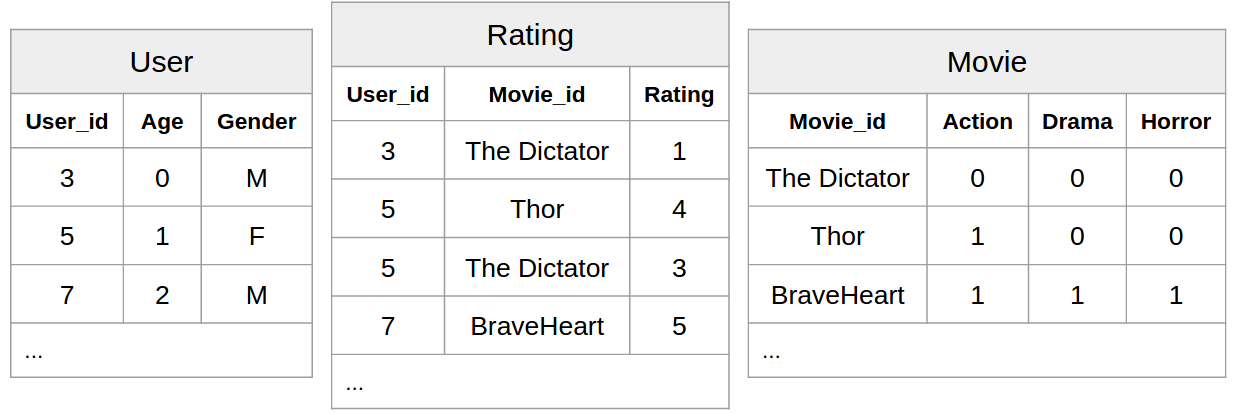
\includegraphics[width=0.48\textwidth] 
	{relExample}
	\caption{Excerpt from a relational dataset/database. 
		\label{fig:database}
		}
\end{figure}








\begin{table}
\caption{Computing the database frequency of a joint assignment to first-order random variables.}
\begin{center}
\resizebox{0.48\textwidth}{!}{
\begin{tabular}{|l|r|r|r|}
\hline
$X = x$ & \multicolumn{1}{l|}{$n(X=x;D)$} & \multicolumn{1}{l|}{$N(X=x;D)$} & \multicolumn{1}{l|}{$P_D(X=x;D)$} \\ \hline
\begin{tabular}{l}Age(User)=0\end{tabular} & 376 & 941 & 0.3996 \\ \hline
\begin{tabular}{l}Age(User)=0,\\ Rating(User,Movie)=1\end{tabular} & 2524 & 1582762 & 0.0016 \\ \hline
\end{tabular}
}
\end{center}
\label{table:frequency}
\end{table}%



\begin{equation} \label{eq:bn}
\ln \bprob{P}{\BN}{\set{\node} = \set{\xvalue}} = \sum_{i=1}^{n} \ln 
\cprob
{P_{\BN}}
{\node_{i} = \set{\xvalue}_{i}}
{
\Pa{i}{\graph} = \pavalue{i}{\graph}
}.
\end{equation}

where $\set{\xvalue}_{i}$ resp. $\pavalue{i}{\graph}$ is the assignment of values to node $\node_{i}$ resp. the parents of $\node_{i}$ determined by the assignment $\set{\xvalue}$. 
%The function $\ln$ is the binary logarithm base 2. 
%To avoid difficulties with $\log(0)$, here and below we assume that joint distributions are positive everywhere. 


\paragraph{Example} Figure~\ref{fig:bn} shows an example of two small Bayesian networks.  The rating value is n/a (for ``not applicable'') if and only if the user has not rated the movie (cf.~\cite{Russell2010}). For the 2-node BN,  Equation~\ref{eq:bn} yields 
\begin{align*}
P(\it{Rating(User,Movie)} = 1, \it{Age(User)} = 1)\\ = 0.00297 \cdot 0.41205 \approx 0.00122.
\end{align*}



\begin{figure}[htbp]
	\centering
	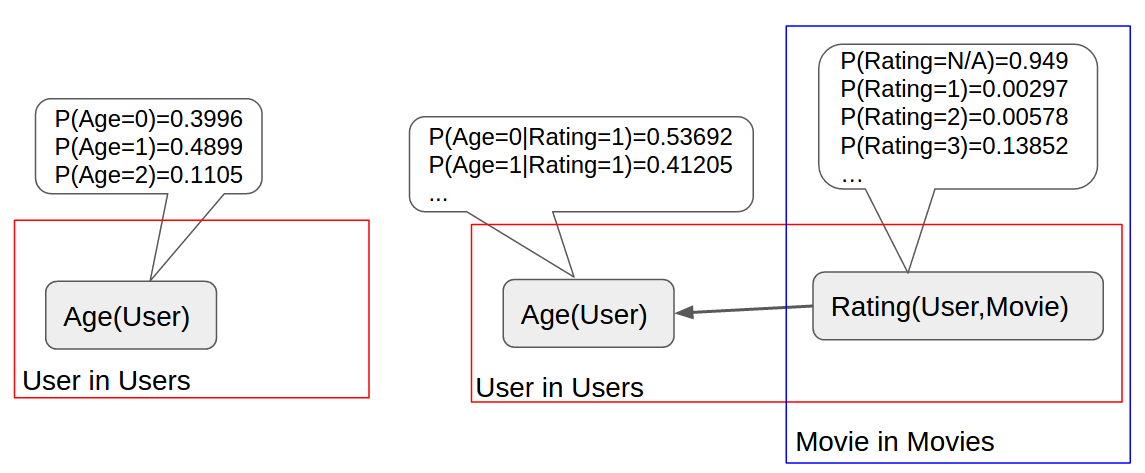
\includegraphics[width=0.48\textwidth] 
	{bnstruct}
	\caption{Example First-Order Bayesian networks. The type of population variables is shown as in a plate model. Conditional probability parameters were estimated from the MovieLens database.
		\label{fig:bn}}
\end{figure}



A first-order Bayesian network (FOB)~\cite{Wang2008}, aka Parametrized BN~\cite{Kimmig2014}, is a Bayesian network whose nodes are first-order terms. Following Halpern's well-known random selection semantics for probabilistic logic, a FOB can be viewed as a model of database frequencies~\cite{Schulte2014}; in the terminology of \cite{Getoor2001a}, a FOB can be used as a Statistical-Relational Model (SRM). The basic idea is to view a population variable as a random selection of individuals from the variable's population. Functors are then functions of random variables, hence themselves random variables. For example, $$P(\it{Rating(User,Movie)} = 1, \it{Age(User)} = 1) = 0.00122$$ can be read as ``if we randomly select a user and a movie, the probability is 0.00122 that the user has age level 1 and rates the movie 1''. The topic of the next section is quantifying how well the joint distribution $\bprob{P}{\BN}{\cdot}$ represented in an SRM via Equation~\eqref{eq:bn} fits the database distribution $\dprob{\dstructure}{\cdot}$ defined by Equation~\eqref{eq:proportion}.

\section{Relational Model Comparison} 

We define the relational  model comparison scores that we study in this paper. We begin with general model selection concepts. 
%The model scores we consider have as components a likelihood function and a complexity penalty term. We consider relational likelihood functions, then how to expand them with terms that penalize model complexity. 
%
\subsection{Model Score Concepts} 

%We adapt previously established notation and concepts  for Bayesian network structure scores. 
A score $\Score{S}{\graph}{\dstructure}$ measures how well a DAG $\graph$ fits a database $\dstructure$~\cite{Chickering2003}.  A \textbf{gain function} $\Gain{\dstructure}{\graph}{\graph'}{\dstructure}$ measures how much an alternative structure $\graph'$ improves a current structure $\graph$. For  every score $S$, there is an associated gain function  defined by $\Gain{\Delta_{S}}{\graph}{\graph'}{\dstructure} = \Score{S}{\graph'}{\dstructure} - \Score{S}{\graph}{\dstructure}$. 
%
%However, there may be gain functions that cannot be represented as a score difference; this is the case for the relational gain functions that we propose in this paper. The scores that we consider in this paper combine a positive log-likelihood term, measuring how well the model fits the data, with a negative penalty term, measuring the data-independent complexity of the model. ~\cite{Bouckaert1995} provides a general survey of such scores. Our discussion focuses on the $\aic$ and $\bic$ scores. These are very widely used scores for statistical model selection, with a simple mathematical form. Our method for adapting $\aic$ and $\bic$ to relational data can be used for other scores as well, for instance BDEu and normalized MDL \cite{score-paper}.
%
A score function is \textbf{decomposable} if it can be written as a sum of local scores $s$, each of which is a function only of one node and its parents; see Equation~\eqref{eq:decompose}. Similarly, a gain function is decomposable if the improvement can be written as a sum of local improvements $\delta$; see Equation~\eqref{eq:decompose-gain}. Many structure search algorithms consider adding the addition or deletion of a single edge at a time \cite{Chickering2003}. Let $\node_{+}\rightarrow \node_{i}$ be an edge not contained in $\graph$, and let $\graph_{+}$ be the graph that adds the edge to $\graph$. In that case we write the local gain only as a function of the previous parents and the new parent $\node_{+}$; see Equation~\eqref{eq:gain-short}. 


\begin{eqnarray}
%\resizebox{0.48\textwidth}{!}{
\label{eq:decompose} \Score{S}{\graph}{\dstructure}&=&\sum_{i} \score{s}{i}{\Pa{i}{\graph}}{\dstructure} \\
\Gain{\Delta}{\graph}{\graph'}{\dstructure}&=& 
\sum_{i} \delta(\node_{i},\Pa{i}{\graph},\Pa{i}{\graph'},\dstructure)  \label{eq:decompose-gain}
\\& = & \gain{\delta}{i}{\graph}{\dstructure} \label{eq:gain-short}
% \Gain{\Delta}{\graph}{\graph'}{\dstructure}& = & \gain{\delta}{i}{\graph}{\dstructure} \label{eq:single-edge-gain}}
\end{eqnarray}


We consider upgrading an i.i.d. score of the form
(log-likelihood of data under model) - (penalty = function of number of parameters, sample size). We first discuss upgrading the log-likelihood term.

\subsection{Relational Model Likelihood Scores}

Whereas the independence of i.i.d. data induces a unique product likelihood function, several BN likelihood functions have been proposed for multi-relational data. The reason is that template BN structures represent multiple dependent instantiations, and there are different approaches to aggregating them; see Section~\ref{sec:related}. We focus on the most recent proposal, {\em log-linear likelihood scores}~\cite{Schulte2011}, whose form is similar to the log-linear likelihood of Markov Logic Networks (Section~\ref{sec:related}). A log-linear likelihood score is a factor product  that is not necessarily normalized (not summing to 1). Log-linearity has the following advantages~\cite{Schulte2011}. (1) Generalizing the i.i.d. case: The mathematical form is very close to the  i.i.d. log-likelihood function for Bayesian networks. (2) Tractability: The score is maximized by the empirical conditional frequencies, as in the i.i.d. case. It can therefore be computed in closed form, given the sufficient statistics in the data. (3) Autocorrelation: The score is well-defined even when the data exhibit cyclic dependencies (see Section~\ref{sec:related}). 


We adopt standard notation for BN sufficient statistics~\cite{Heckerman1998}. Let $\node_{i} = \xvalue_{ik},\Pa{i}{\graph}=\pavalue{ij}{\graph}$ be the assignment that sets node $i$ to its $k$-th value, and its parents to their $j$-th possible configuration. We associate the following concepts with the $ijk$ assignment.


\begin{itemize}
\item $\Fcount{\graph}{ijk}{\dstructure} \equiv \Count{\node_{i} = \xvalue_{ik},\Pa{i}{\graph}=\pavalue{ij}{\graph}}{\dstructure}$ is the number of groundings that satisfy the $ijk$ assignment.
\item $\Fcount{\graph}{ij}{\dstructure} \equiv \sum_{k} \Fcount{\graph}{ijk}{\dstructure}$ is the number of groundings that satisfy the $j$-th parent assignment.
\item $\Fcount{\graph}{i}{\dstructure} \equiv \sum_{j}\sum_{k} \Fcount{\graph}{ijk}{\dstructure}$ is the number of possible groundings for node $i$.
\end{itemize}
The number of possible groundings can be directly computed as the product of the sample size $\varsize{\Avariable}{\dstructure}$  associated with each population variable $\Avariable$ that is contained in node $i$ or its parents. 
%
%\begin{equation} \label{eq:local-sample}
%\Fcount{\graph}{i}{\dstructure} = \varsize{\Avariable_{1}}{\dstructure} \times \cdots \times \varsize{\Avariable_{m}}{\dstructure}.\end{equation}
%
%where $\varsize{\Avariable}{\dstructure}$ is the size of the sample population associated with variable $\Avariable$.
Since the quantity $\Cvar_{i}^{\graph}$ plays the same role as the sample size in i.i.d. data, we refer to it as the \defterm{local sample size} for node $i$. 
%(Even though the groundings associated with node $i$ do not form an i.i.d. random sample.) 
A key difference is that the {\em local sample size $\Cvar_{i}^{\graph}$ depends on both the data and the graph structure}~\cite{Lowd2007}. In contrast, the global sample size $\Cvar$ in i.i.d. data is the same for all nodes and for all graphs. 
%Within a graph, different nodes can be associated with exponentially different local sample sizes, a form of ill-conditioning \cite{Lowd2007}. 
%Across graphs, adding/deleting an edge induces an exponential change in the local sample size if population variables are added/subtracted from a local family [cite foil-gain?]. 
The question of how to compare models with different local sample sizes is the main question of this paper.

Table~\ref{table:ll} gives the formulas for two previously proposed relational log-likelihood scores. The \defterm{count log-likelihood} has the same form as the local log-likelihood for i.i.d. data, but replaces counts in a single data table by counts in a database. The \defterm{frequency likelihood}~\cite{Schulte2011} normalizes the count score by the local sample size (see also \cite{Xiang2011}). This is equivalent to replacing counts in a single data table by frequencies in a database. 




\begin{table}
\caption{Relational Local (Pseudo) Log-likelihood Scores.}
\begin{center}
\resizebox{0.48\textwidth}{!}{
\begin{tabular}{|c|c|c|}
\hline
Name & Symbol & Definition \\\hline
Count & $\score{\cscore{\loglikelihood}}{i}{\Pa{i}{\graph}}{\dstructure} $& $ \sum_{j} \sum_{k} \Fcount{\graph}{ijk}{\dstructure} \cdot \log_{2} \left( \frac
{\Fcount{\graph}{ijk}{\dstructure}}
{\Fcount{\graph}{ij}{\dstructure}}\right)  $ \\\hline
Frequency & $\score{\nscore{\loglikelihood}}{i}{\Pa{i}{\graph}}{\dstructure}$& $1/\Fcount{\graph}{i}{\dstructure} \times \score{\cscore{\loglikelihood}}{i}{\Pa{i}{\graph}}{\dstructure}$
%$ 1/\Fcount{\graph}{i}{\dstructure} \sum_{j} \sum_{k} \Fcount{\graph}{ijk}{\dstructure} \cdot 
%\ln 
%\left(\frac
%{\Fcount{\graph}{ijk}{\dstructure}}
%{\Fcount{\graph}{ij}{\dstructure}}
%\right)  
\\\hline
\end{tabular}}
\end{center}
\label{table:ll}
\end{table}%


For i.i.d. data, adding an edge to a graph $\graph$ can only increase the log-likelihood score. A big difference to the relational case is that {\em adding an edge can decrease the relational count log-likelihood.} This occurs when the new edge \defterm{adds a population variable} that was not contained in the child node or the previous parents; see Figure~\ref{fig:bn} and Table~\ref{table:likelihood-example}. In contrast, adding an edge cannot decrease the frequency log-likelihood. Table~\ref{table:likelihood-example} illustrates the computations of the different log-likelihood scores.%We refer to such an edge as an \defterm{expanding} edge, and to its opposite as a \defterm{contained} edge. In contrast, adding an edge, of either type, can only increase the frequency log-likelihood. 

% \begin{figure}[thbp]
% 	\centering
% 	\includegraphics[width=0.5\textwidth] 
% 	{missing}
% 	\caption{A population-adding edge to expand a structure $\graph$ to a larger structure $\graph_{+}$. (a) A CP-table for $\graph$. (b) A CP-table for $\graph_{+}$. (c) 	A CP-table for $\graph_{+}$ that ignores the new parent. The parameter values are maximum likelihood estimates computed from the IMDb database.\label{fig:likelihood-example}}
% \end{figure}

\begin{table}
\resizebox{0.48\textwidth}{!}{
\begin{tabular}{|l|r|l|r|r|r|r|r|}
\hline
Family Configuration & \multicolumn{1}{l|}{$n_{ijk}$} & $n_{ij}$ & \multicolumn{1}{l|}{$n_{i}$} & \multicolumn{1}{l|}{$n_{ijk}/n_i$} & \multicolumn{1}{l|}{\emph{CP}} & \multicolumn{1}{l|}{$L$} & \multicolumn{1}{l|}{$\overline{L}$} \\ \hline
\begin{tabular}{l}Age(User)=0\end{tabular} & 376 & --- & 941 & 0.3996 & 0.3996 & -497.6217 & -0.5288 \\ \hline
\begin{tabular}{l}Age(User)=0, \\Rating(User,Movie)=1\end{tabular} & 2524 & \multicolumn{1}{r|}{4703} & 1582762 & 0.0016 & 0.5367 & -2266.2224 & -0.0014 \\ \hline
\end{tabular}
}
\caption{A population-adding edge to expand a structure $\graph$ to a larger structure $\graph_{+}$. CP-table for $\graph$ and $\graph_{+}$. The parameter values are maximum likelihood estimates computed from the Movielens database. The $L$ and $\overline{L}$ columns show  the contributions of the family configuration in each row (part of the sum for the total likelihood values).
\label{table:likelihood-example}
}
\end{table}


%\paragraph{Example.} Table~\ref{table:counts} illustrates the different sufficient statistics associated with different BN structures. 
%
%\begin{table}[htdp]
%\caption{Counts and Local Relational Log-likelihood Computations. [Use groundings table?]}
%\begin{center}
%\begin{tabular}{|c|c|}
%Node & Quantity
%\end{tabular}
%\end{center}
%\label{table:counts}
%\end{table}%
%



\subsection{The Normalized Gain Function} \label{sec:gain}
{\em Here and below, we write $\graph_{+}$ for the DAG that results from adding a generic edge $\node_{+} \rightarrow \node_{i}$ to DAG $\graph$.}
Our upgrade method for defining a relational gain function is as follows. 
\begin{enumerate}
\item Compute the likelihood differential using the frequency likelihood $\nscore{\loglikelihood}$.
\item  Normalize the penalty term differential by the {\em larger} sample size $\Fcount{+}{i}{\dstructure}$. 
\item The \defterm{normalized gain} is computed as (1) minus (2), likelihood differential minus penalty differential. 
\end{enumerate}

Table~\ref{table:gains} gives the normalized gain formulas for upgrading the standard $\aic$ and $\bic$ scores~\cite{bouckaert95:_bayes}. (We omit a constant factor of 2 that does not affect model comparisons.) The upgrade method can be applied with other i.i.d. scores as well. We focus on $\aic$ and $\bic$ because of their relatively simple form. Table~\ref{table:compute-scores} shows 
example values for the normalized gains. These are compared with gains based on natural single model scores, which we introduce in the next section.
%Below we show that this gain function cannot be represented in terms of a single model selection score.
%They each normalize both the likelihood difference {\em and} the complexity difference of two candidate models $\graph$ and an expansion $\graph'$. 
%
%There are two possible local sample sizes for normalizing: $\Fcount{\graph}{i}{\dstructure}$ and $\Fcount{\graph'}{i}{\dstructure}$. 

%As we show below, our 
%formulas normalize the local score difference by {\em the sample size associated with the larger graph}, which potentially contains more population variables. This means that the normalization term for the smaller graph depends on which larger graph it is compared to; therefore our relational gain functions cannot be expressed as differences of a single fixed score.

\begin{table*}[htbp] \centering
%\resizebox{0.48\textwidth}{!}{
\begin{tabular}{| c | c |}
	 \hline Local Gain Function & Definition \\ \hline
$\gain{\improve{\nscore{\loglikelihood}}}{i}{\graph}{\dstructure}$ & 
$\score{\nscore{\loglikelihood}}{i}{\Pa{i}{\graph}\cup\node_{+}}{\dstructure} -
\score{\nscore{\loglikelihood}}{i}{\Pa{i}{\graph}}{\dstructure} $
\\ \hline
$\gain{\improve{\nscore{\aic}}}{i}{\graph}{\dstructure}$ & 
$\gain{\improve{\nscore{\loglikelihood}}}{i}{\graph}{\dstructure} - \frac{\parloss{i}{\graph}}{\Fcount{+}{i}{\dstructure}}$
\\ \hline
$\gain{\improve{\nscore{\bic}}}{i}{\graph}{\dstructure}$ & $\gain{\improve{\nscore{\loglikelihood}}}{i}{\graph}{\dstructure} - \frac{\frac{1}{2}\log_{2}(\Fcount{+}{i}{\dstructure}) \parloss{i}{\graph}}{\Fcount{+}{i}{\dstructure}}$
\\ \hline
\end{tabular}
%}
\caption{Our Proposed Normalized Relational Model Gain Upgrade for $\aic$ and $\bic$. $\Fcount{+}{i}{\dstructure} \equiv \Fcount{\graph_{+}}{i}{\dstructure}$ denotes the local sample size for the expanded graph. $\parloss{i}{\graph} = \numpars{\graph^{+}}{i} - \numpars{\graph}{i}$ \label{table:gains}}
\end{table*}

\section{Comparison Multi-Relational \\Model Scores} \label{sec:scores}

The baseline methods  define relational scores by normalizing the likelihood term and/or the penalty term. This upgrade scheme defines 4 different relational versions of a model selection score; see Table~\ref{table:compare-design}. Normalizing the penalty term but not the likelihood term is clearly inadequate. Table~\ref{table:comparison-scores} gives the formulas for the remaining 3 different relational versions of $\aic$ and $\bic$. Table~\ref{table:compute-scores} shows example values. 

\begin{table} \caption{Available options for each score, depending on whether rescaling the likelihood count and/or the penalty term. %Nonconsistency is discussed in Section~\ref{sec:theory}.
} 
\label{table:compare-design}
\resizebox{0.48\textwidth}{!}{
\begin{tabular}{| c | c | c |}
	\hline 	\diagbox{Likelihood}{Penalty} & Count & Normalized
	\\ \hline 
	Count & S; not consistent; underfits & --- 
	\\\hline
	Normalized &  $\widetilde{S}$;  not consistent; underfits & $\overline{S}$; not consistent; overfits
	\\\hline
\end{tabular}
}
\end{table}


\begin{table*} 
\resizebox{1\textwidth}{!}{
\begin{tabular}{| c | c | c |}
	\hline Score & $\aic_{i}$ & $\bic_{i}$ 
%	 $\loglikelihood$
%& $\dlogcount{\graph}{i}{\dstructure} \equiv \sum_{j} \sum_{k}  
%\Fcount{\graph}{ijk}{\dstructure}
%\cdot \ln \left( \frac
%{\Fcount{\graph}{ijk}{\dstructure}}
%{\Fcount{\graph}{ij}{\dstructure}}\right)$
%& $\dlogfreq{\graph}{i}{\dstructure}$
\\\hline
Count-Count
& 
$\score{\cscore{\aic}}{i}{\Pa{i}{\graph}}{\dstructure} \equiv \score{\cscore{\loglikelihood}}{i}{\Pa{i}{\graph}}{\dstructure} - \numpars{\graph}{i}$ 
& 
$\score{\cscore{\bic}}{i}{\Pa{i}{\graph}}{\dstructure} \equiv \score{\cscore{\loglikelihood}}{i}{\Pa{i}{\graph}}{\dstructure} - \frac{1}{2}\log_2(\Fcount{\graph}{i}{\dstructure}) \cdot \numpars{\graph}{i}$

\\\hline
Normalized-Normalized
&
$\score{\nscore{\aic}}{i}{\Pa{i}{\graph}}{\dstructure} \equiv \frac{1}{\Fcount{\graph}{i}{\dstructure}} \score{\cscore{\aic}}{i}{\Pa{i}{\graph}}{\dstructure}$
&
$\score{\nscore{\bic}}{i}{\Pa{i}{\graph}}{\dstructure} \equiv \frac{1}{\Fcount{\graph}{i}{\dstructure}} \score{\cscore{\bic}}{i}{\Pa{i}{\graph}}{\dstructure}$

\\\hline
Normalized-Count
&
$\score{\ncscore{\aic}}{i}{\Pa{i}{\graph}}{\dstructure} \equiv \score{\nscore{\loglikelihood}}{i}{\Pa{i}{\graph}}{\dstructure} - \numpars{\graph}{i}$
&
$\score{\ncscore{\bic}}{i}{\Pa{i}{\graph}}{\dstructure} \equiv \score{\nscore{\loglikelihood}}{i}{\Pa{i}{\graph}}{\dstructure} - \frac{1}{2}\log_2(\Fcount{\graph}{i}{\dstructure}) \cdot \numpars{\graph}{i}$
\\\hline
\end{tabular}
} % end box
\caption{Relational Local Model Selection Scores, count and frequency versions. Normalized scores divide count scores by the local sample size $\Fcount{\graph}{i}{\dstructure}$.} \label{table:comparison-scores}
\end{table*}

\begin{table*}
% \begin{tabular}[c]{r|r|r|r|r|r|r|r|r|r|r|r}
% conf & \#parameters & L & L-bar & AIC & BIC & AIC & BIC & AIC & BIC & AIC & BIC \\
% $\graph$ & 2 & -497.62 & -0.53 & -26055.19 & -26067.39 & -1.38 & -1.39 & -3.38 & -15.58 & --- & --- \\
% $\graph^{+}$  & 12 & -2266.22 & 0.00 & -43802563.66 & --- & -1.38 & -1.38 & -13.38 & -150.88 & --- & --- \\
% GAIN &  & -1768.60 & 0.53 & -43776508.47 & \#VALUE! & 0.00 & 0.00 & -10.00 & -135.30 & g:-1.3844416518832763 g+:-1.3836674348843243 & g:-1.3850898973140742 g+:-1.3812350552292387
% \end{tabular}

%SUBMITTED CIKM TABLE:
% \resizebox{1\textwidth}{!}{
% \begin{tabular}{|l|c|c|c|c|c|c|c|c|c|c|c|c|}
% \hline
%  & \multicolumn{1}{l|}{} & \multicolumn{1}{l|}{} & \multicolumn{1}{l|}{} & \multicolumn{1}{c|}{} & \multicolumn{4}{c|}{AIC} & \multicolumn{4}{c|}{BIC}  \\ \hline
%  & \multicolumn{1}{l|}{\#groundings} & \multicolumn{1}{l|}{\#parameters} & \multicolumn{1}{l|}{L} & \multicolumn{1}{l|}{$\overline{L}$} & \multicolumn{1}{l|}{count-count} & \multicolumn{1}{l|}{normalized-normalized} & \multicolumn{1}{l|}{normalized-count} & normalized gain & \multicolumn{1}{l|}{count-count} & \multicolumn{1}{l|}{normalized-normalized} & \multicolumn{1}{l|}{normalized-count} & normalized gain \\ \hline
% G & 941.00 & 2.00 & -27.7 & -0.02944 & -29.70 & -0.03156 & -2.03 & --- & -37.58 & -0.0399 & -9.91 & --- \\ \hline
% G+ & 1582762 & 12 & -27.6 & -0.00002 & -39.60 & -0.00003 & -12.00 & --- & -151.16 & -0.0001 & -123.56 & --- \\ \hline
% GAIN &  & 10 & 0.1 & 0.02942 & -9.90 & 0.03154 & -9.97 & 0.02941 & -113.59 & 0.0398 & -113.66 & 0.02935 \\ \hline
% \end{tabular}


\resizebox{1\textwidth}{!}{
\begin{tabular}{|l|c|c|c|c|c|c|c|c|c|c|c|c|}
\hline
 & \multicolumn{1}{l|}{} & \multicolumn{1}{l|}{} & \multicolumn{1}{l|}{} & \multicolumn{1}{c|}{} & \multicolumn{4}{c|}{AIC} & \multicolumn{4}{c|}{BIC}  \\ \hline
 & \multicolumn{1}{l|}{\#groundings} & \multicolumn{1}{l|}{\#parameters} & \multicolumn{1}{l|}{L} & \multicolumn{1}{l|}{$\overline{L}$} & \multicolumn{1}{l|}{count-count} & \multicolumn{1}{l|}{normalized-normalized} & \multicolumn{1}{l|}{normalized-count} & normalized gain & \multicolumn{1}{l|}{count-count} & \multicolumn{1}{l|}{normalized-normalized} & \multicolumn{1}{l|}{normalized-count} & normalized gain \\ \hline
G & 941 & 2 & -1302.7 & -1.384 & -1304.7 & -1.3865 & -3.38 & --- & -1312.5 & -1.3948 & -11.26 & --- \\ \hline
G+ & 1582762 & 12 & -1863691.4 & -1.177 & -1863703.4 & -1.1775 & -13.18 & --- & -1863814.9 & -1.1776 & -124.74 & --- \\ \hline
GAIN &  & 10 & -1862388.7 & 0.207 & -1862398.7 & 0.2090 & -9.79 & 0.20684 & -1862502.4 & 0.2173 & -113.48 & 0.20678 \\ \hline
\end{tabular}



% \begin{tabular}{|l|l|r|r|r|r|r|r|r|r|l|l|}
% \hline
%  &  & \multicolumn{2}{c|}{Likelihood} & \multicolumn{2}{c|}{Count}& \multicolumn{2}{c|}{Normalized}& \multicolumn{2}{c|}{Weighted}& \multicolumn{2}{c|}{Normalized Gain}  \\ \hline
% Family Configuration & \#parameters & \multicolumn{1}{l|}{$L$} & \multicolumn{1}{l|}{$\overline{L}$} & \multicolumn{1}{l|}{AIC} & \multicolumn{1}{l|}{BIC} & \multicolumn{1}{l|}{AIC} & \multicolumn{1}{l|}{BIC} & \multicolumn{1}{l|}{AIC} & \multicolumn{1}{l|}{BIC} & AIC & BIC \\ \hline
% $\graph$ & \multicolumn{1}{r|}{2.00} & -902.94 & -0.95 & -26055.2 & -26067.4 & -1.3844 & -1.3851 & -3.38 & -15.58 & --- & --- \\ \hline
% $\graph^{+}$ & \multicolumn{1}{r|}{12.00} & -1518082.25 & -0.96 & -43802563.7 & -43725109.0 & -1.3837 & -1.3837 & -13.38 & -150.88 & --- & --- \\ \hline
% GAIN & -10.00  & -1517179.3 & -0.01 & -43776508.5 & -43699041.6 & 0.0007 & 0.0013 & -10.00 & -135.30 & \multicolumn{1}{r|}{0.0008} & \multicolumn{1}{r|}{0.0039} \\ \hline
% \end{tabular}
}
\caption{Example Values for the Scores and Gain Functions defined in this section. For the structures of Figure \ref{fig:bn}. \label{table:compute-scores}}
\end{table*}

%

The next proposition establishes that the normalized gain function defines a new concept, in that it cannot be represented as a difference of single  model selection scores. In fact, we give a stronger result: no scaled version of the normalized gain function can be represented as a difference associated with a single  model selection score. A scaling corresponds to a {\em unit change} that can be represented as a positive linear transformation $[\alpha \mbox{ (normalized gain) } + c]$ where $\alpha > 0$ may depend only on the local sample sizes of the structures compared. 

\begin{proposition} \label{prop:balance}
There is no relational model selection score such that its associated model gain function is a unit change applied to the normalized gain function.
\end{proposition}

We omit the proof. Intuitively, the reason is that a balanced gain function has to adjust the score of the smaller graph $\graph$ depending on whether the new edge $\node_{+} \rightarrow \node_{i}$ adds a population variable or not. This is impossible if the score for $\graph$ is fixed. {\em The proposition shows that no balanced log-linear gain function is representable in terms of a log-linear single model selection score.} Our argument for this conclusion is as follows. The normalized gain is balanced because the likelihood scores and the penalty terms are standardized to the same scale. Therefore any balanced log-linear gain function should be a scaling (unit change) of the normalized gain. (Much like any valid temperature scale is a unit change of the centigrade scale.) Thus Proposition~\ref{prop:balance} should apply to any balanced log-linear gain function. 

\paragraph{Example} Consider the {\em rescaled gain function} $[\Fcount{+}{i}{\dstructure} \times \mbox{ (normalized gain)}].$ This is equivalent to the following upgrade procedure. (1) Multiply the count likelihood for the smaller graph $\graph$ by the factor $\frac
	{\Fcount{+}{i}{\dstructure}}
	{\Fcount{\graph}{i}{\dstructure}}$. Since the term $\frac
	{\Fcount{+}{i}{\dstructure}}
	{\Fcount{\graph}{i}{\dstructure}}$ represents the number of possible groundings added by the expansion $\graph_{+}$, this puts the count likelihoods for both graphs on the same scale. 
%	(2) Normalize all count likelihood and penalty terms by the local sample size for the larger graph $\graph_{+}$. 
	(2) Return the resulting score differential. For instance, the rescaled gain function for AIC is given by the formula
\scriptsize
	$$\score{\loglikelihood}{i}{\Pa{i}{\graph}\cup\node_{+}}{\dstructure} -
\left(\frac
	{\Fcount{+}{i}{\dstructure}}
	{\Fcount{\graph}{i}{\dstructure}} \times \score{\loglikelihood}{i}{\Pa{i}{\graph}}{\dstructure} \right) - \parloss{i}{\graph}.$$
	
	\normalsize
	
	
	The rescaled gain function is balanced, since counts and parameters are measured on the same scale. Proposition~\ref{prop:balance} entails that the rescaled gain function cannot be represented by a single model selection score. Conversely, the log-linear single model selection scores of Table~\ref{table:comparison-scores} are not balanced. As we show in the next section, their lack of balance leads to nonconsistency.


\section{Consistency Analysis} \label{sec:theory}
%$\node_{+} \rightarrow \node_{i}$
This section shows that the normalized gain function is relatively consistent, but the model score functions are not. The reason is that the former are balanced and the latter are not. We observe that (*)  {\em for edges that do not add population variables, the normalized gain, the count-count, and the normalized-normalized comparisons are equivalent.}
 This is because in this case the local sample sizes are the same for both structures (i.e., $\Fcount{\graph}{i}{\dstructure} = \Fcount{+}{i}{\dstructure}$). Therefore our analysis focuses on the case where the model comparisons differ: edges that do add population variables.

\subsection{Local Consistency} A large sample analysis considers a sequence of samples from the true data generating distribution that grow without bound. A model selection method is consistent if the sequence of models that it selects converges to one that is correct for the data generating distribution. Following previous work on consistency for relational data~\cite{Sakai2013,Xiang2011,Shalizi2013}, we formalize these concepts as follows. In the limit the sample size for each population $\individuals_{i}$ goes to infinity, 
%$\psize{\individuals_{i}}{\dstructure_{j}} \rightarrow \infty$, 
which like \cite{Sakai2013} we 
%abbreviate 
denote as $$\set{\samplesize}(\dstructure) \rightarrow \infty.$$  Like \cite{Xiang2011}, we make the identifiability assumption that  $$\dprob{\dstructure}{\cdot}\rightarrow\dprob{\structure}{\cdot} \equiv p  \mbox{ as } \set{\samplesize}(\dstructure) \rightarrow \infty.$$ Here $\structure$ represents a complete relational structure (network) from which samples are drawn. We abbreviate the frequency distribution associated with the complete structure as $p$, for brevity and compatibility with \cite{Chickering2003} where $p$ is used for the data generating distribution.
%
 Arbitrarily large samples can be generated either by sampling with replacement, or by sampling from infinite populations.  For  discussion of network sampling, see \cite{Shalizi2013,Frank1977}. The definition of the relational frequency $\dprob{\structure}{\cdot}$ with infinite populations is given in \cite{Halpern90}.
%
%Let $\dstructure_{1},\ldots,\dstructure_{j},\ldots$ be a sequence of databases sampled from structure $\structure$. The data sequence \defterm{converges} if, as $j \rightarrow \infty$,
%
%\begin{enumerate}
%\item $\dprob{\dstructure_{j}}{\cdot}\rightarrow\dprob{\structure}{\cdot} \equiv p$, and [state this as assumption]
%\item $\psize{\individuals_{i}}{\dstructure_{j}} \rightarrow \infty$ for each population $\individuals_{i}$. We abbreviate this as $\set{\samplesize} \rightarrow \infty$.\footnote{Arbitrarily large samples can be generated either by sampling with replacement, or by sampling from infinite populations. The definition of the relational frequency $\dprob{\structure}{\cdot}$ with infinite populations is worked out by \cite{Halpern1990}. The basic idea is to assume that $\structure$ defines a probability measure over tuples of individuals, so the probability $\dprob{\structure}{\set{\Xvariable} = \set{\xvalue}}$ of an assignment is the mass of the set of groundings that satisfy the assignment.}
%\end{enumerate}
%
%A BN structure learning method method is consistent if in the large sample limit, the graph it selects is an I-map for $p$. This means that there is a Bayesian network $\BN =  (\graph,\set{\parameter})$ such that $\dprob{\BN}{\cdot} = p(\cdot)$.
Chickering and Meek analysed BN model selection scores in terms of \defterm{local consistency}, which we adapt for score gain functions as follows.

\begin{definition}
% Let $\dstructure$ be a database with sample size vector $\set{\samplesize}$, and 
 Let $p$ be the data generating distribution. A local gain function is \defterm{locally consistent} if, the following hold in the sample size limit as $\set{\samplesize}(\dstructure) \rightarrow \infty$, for any single-edge expansion $\graph_{+}$:

%\begin{enumerate}
%\item If $\node_{+}$ is not independent of $\node_{i}$ given  $\Pa{i}{\graph}$ in $\dprob{\structure}{\cdot}$, then $\Gain{\Delta}{\graph}{\graph_{+}}{\dstructure_{m}} > 0$.
%\item If $\node_{+}$ is independent of $\node_{i}$ given  $\Pa{i}{\graph}$ in $\dprob{\structure}{\cdot}$, then $\Gain{\Delta}{\graph}{\graph_{+}}{\dstructure_{m}} < 0$.
%\end{enumerate}


\begin{enumerate}
\item If $\node_{+}$ is not independent of $\node_{i}$ given  $\Pa{i}{\graph}$ in $p$, then \\$\Gain{\Delta}{\graph}{\graph_{+}}{\dstructure} > 0$.
\item If $\node_{+}$ is independent of $\node_{i}$ given  $\Pa{i}{\graph}$ in $p$, then \\$\Gain{\Delta}{\graph}{\graph_{+}}{\dstructure} < 0$.
\end{enumerate}

\end{definition}
%
%The first property states that the score favors adding any edges that represent a true dependency. The second property states that the score favors eliminating any  edges that do not represent a true dependency.
%
%Local consistency implies global consistency, in the sense that any gain-optimal graph represents the true distribution. A graph $\graph$ is \defterm{gain-optimal} for a data set $\dstructure$ if there is no other graph $\graph'$ such that $\Gain{\Delta}{\graph}{\graph'}{\dstructure} > 0$. 
%\begin{proposition}
%If a gain function is locally consistent, it is consistent. That is, as $\set{\samplesize} \rightarrow \infty$, any gain-optimal graph $\graph$ for a dataset $\dstructure$ is an I-map for $p$. 
%\end{proposition}
%{\em Proof.} Standard results in Bayes net theory imply that if a graph structure $\graph$ is not an I-map for $\dprob{\structure}{\cdot}$, then there is an edge $\node_{+} \rightarrow \node_{i}$ such that $\node_{+}$ is not independent of $\node_{i}$ given  $\Pa{i}{\graph}$ in $\dprob{\structure}{\cdot}$. Thus by the first property of local consistency, adding the edge leads to a positive gain, so the graph $\graph$ is not gain-optimal.
%
%The second property of local consistency implies that only an edge-minimal I-map \cite{Pearl} $\graph$ is gain-optimal, meaning that no proper subgraph of $\graph$ is an I-map for $\dprob{\structure}{\cdot}$. Chickering and Meek examine in detail the connection between local consistency and optimal graph structures. In the following we focus on whether gain functions are locally consistent.

%\subsection{Consistency of the Relational Model Gain} This section establishes the local consistency of the relational model gain score. The key step in 
 
The first clause requires that edges that represent valid dependencies receive a positive gain. The second clause requires that redundant edges that do no represent a valid dependency receive a negative gain. An upgrade method is relatively locally consistent if the upgraded i.i.d. gain function (which may be derived from a single score) is locally consistent for relational data, whenever it is locally consistent for i.i.d. data.
 
\begin{theorem} \label{th:consistency}
The normalized gain function (Section~\ref{sec:gain})  is relatively locally consistent. 
None of the relational model scores (Section~\ref{sec:scores}) are relatively locally consistent.
\end{theorem}
 
{\em Proof.} Case 1: The additional edge $\node_{+} \rightarrow \node_{i}$ adds no population variables. For such edges, the count-count upgrade score  has the same mathematical form as the original i.i.d. score. Therefore the arguments of~\cite{Chickering2003} apply, and the score is locally consistent. Since by (*), for such edges, the normalized gain is equivalent to the count-count upgrade score, 
%simply scales the count-count score difference by the local sample size $\Fcount{+}{i}{\dstructure}$, 
the normalized gain is locally consistent as well. 

Case 2: The additional edge $\node_{+} \rightarrow \node_{i}$ adds a population variable. For concreteness, assume that the edge is of the form $g(\Avariable,\Bvariable) \rightarrow f(\Avariable)$, so the added sample size is $\varsize{\Bvariable}{\dstructure}$. Consider a transformed database $\dstructure'$ where $f(\Avariable)$ is replaced by $f'(\Avariable,\Bvariable)$, with an inert second argument: $f'(\aconstant,\bconstant) = f(\aconstant)$. Then in $\dstructure'$, each satisfying assignment in $\dstructure$ for the family of $f(\Avariable)$  is multiplied by $\varsize{\Bvariable}{\dstructure}$. Therefore the sufficient statistics are related as follows: 
$$\Fcount{\graph}{ijk}{\dstructure'} = 
\varsize{\Bvariable}{\dstructure} \times\Fcount{\graph}{ijk}{\dstructure}$$ and $$\Fcount{\graph_{+}}{ijk}{\dstructure'} = 
\Fcount{\graph_{+}}{ijk}{\dstructure}.$$ These equalities imply that the normalized gain for $\dstructure$ is the same as that for $\dstructure'$. Now in $\dstructure'$, the new edge adds no population variables, and so by Case 1, the normalized gain is locally consistent for $\dstructure'$. Therefore it is locally consistent for $\dstructure$. Hence in either case, the normalized gain is locally consistent.


For the non-consistency, we omit a formal proof due to space constraints. Instead, we give the intuitive reason. 
%From this intuition, we derive the following hypotheses that we evaluate in our experiments.
By under(over)fitting we mean producing an overly sparse (dense) DAG.

\begin{description}
\item[Count-Count Score $S$]  The count likelihood typically decreases for an edge that adds a population variable, even if the edge represents a true dependency. We expect to observe {\em underfitting}.
\item[Normalized-Count $\widetilde{S}$] The weight of the likelihood term does not increase with sample size, so an edge that represents a true dependency may not be added even in the sample size limit. We expect to observe {\em underfitting}.
\item[Normalized-Normalized $\overline{S}$] The normalized penalty term for the expanded structure $\graph_{+}$ is downweighted more than the normalized penalty term for the simpler structure $\graph$. So a redundant edge may be added even in the sample size limit. We expect to observe {\em overfitting.} 
\end{description}



%Hypothesis 1: Count Score  This effect should be very strong.
%
%Hypothesis 2: The Weighted Score This effect should be weaker than for hypothesis 1.

%Hypothesis 3: The Normalized Score overfits because the normalized penalty term for the more complex structure approaches 0 more quickly than the normalized penalty term for the simpler structure.
From the insights in this section, we derive a number of empirical hypotheses about the relationships between the upgrade methods. 

\subsection{Hypotheses} We assess these hypotheses in experiments that are described in the following section.

\begin{enumerate}
\item A normalized-count score selects smaller graphs than the other upgrade methods. \label{hyp:weighted}
\item A normalized-normalized score selects larger graphs than the other upgrade methods.\label{hyp:normalized} 
\item A count-count score does not select edges that add population variables. \label{hyp:noadd}
\item The difference between upgrade methods concern only edges that add population variables. \label{hyp:contained}
%\item If most nodes represent unary attributes, then most edges are contained edges.\label{hyp:contained-most}
\end{enumerate}

%The first three hypotheses follow from the log-likelihood and penalty scales described in the previous subsection. Hypothesis~\ref{hyp:contained} follows from observation (*). The reason for hypothesis~\ref{hyp:contained-most} is that {\em if two unary attributes contain different population variables, they are marginally independent.} For example, the nodes $\it{gender}{\it{Actor}}$ and $\it{genre}(\it{Movie})$ are marginally independent because the attributes of a randomly selected actor are independent of those of a randomly selected Movie. The nodes may be conditionally dependent given that the actor appeared in the movie, that is, given $\it{AppearsIn}(\it{Actor},\it{Movie}) = \true$. However, a BN score favors a v-structure $$\it{gender}{\it{Actor}} \rightarrow \it{AppearsIn}(\it{Actor},\it{Movie}) \leftarrow \it{genre}(\it{Movie})$$ for representing this (in)dependence pattern. No edge in this v-structure adds population variables. 





\section{Evaluation} 


We describe the system and the datasets we used.
Code was written in Java, JRE 1.7.0.  and executed with 8GB of RAM and a single Intel Core 2 QUAD Processor Q6700 with a clock speed of 2.66GHz (no hyper-threading). The operating system was Linux Centos 2.6.32. 
The MySQL Server version 5.5.34 was run with 8GB of RAM and a single core processor of 2.2GHz. 
All code and data is available on-line (pointer removed for blind review).

\subsection{Datasets} 
We used seven benchmark real-world databases from the CTU Prague Relational Learning Repository~\cite{Motl2015a}. For detailed descriptions and  the sources of the databases, please see references~\cite{Schulte2012,Qian2014a}. Table~\ref{table:datasetsize} summarizes basic information about the benchmark datasets.   IMDb is the largest dataset in terms of number of total tuples (more than 1.3M tuples) and schema complexity. %attributes.
It combines the MovieLens database\footnote{www.grouplens.org, 1M version} with data from the Internet Movie Database (IMDb)\footnote{www.IMDb.com, July 2013} following \cite{Peralta2007}.

\begin{table} \centering
%\scalebox{0.7in}{
\resizebox{0.48\textwidth}{!}{
\begin{tabular}[c]
{|l|c|c|r|c|}\hline
 \textbf{Dataset} & \textbf{\begin{tabular}[l] {ll} \#Relationship \\Tables/ Total \end {tabular}} & \textbf{\#Tuples} & \textbf{\#Attributes}  \\\hline
% \textbf{Dataset} & \textbf{Relationships} & \textbf{\begin{tabular}[l] {ll} Self \\Relationships \end {tabular}} &
% \textbf{\begin{tabular}[l] {ll} Same Type\\ Relationships \end {tabular}}& \textbf{\#Tuples} & \textbf{\begin{tabular}[l] {ll} \#Attribute  \\Columns \end{tabular}}  \\\hline
 University&2 & 171 & 12\\\hline
    Movielens &1 / 3   & 1,010,051 & 7\\\hline
%    Movielens(0.1M) &1 & N & N &  83,402 & 7\\\hline
    Mutagenesis & 2 / 4 & 14,540 & 11\\\hline
    Financial &3 / 7   &  225,932& 15\\\hline
   Hepatitis &3 / 7  &12,927  & 19\\\hline
   IMDb &3 / 7  &1,354,134  & 17\\\hline 
\end{tabular}
}
 % end scalebox
\caption{Datasets characteristics. \#Tuples = total number of tuples over all tables in the dataset. 
  \label{table:datasetsize}}
\end{table}


\subsection{Methods Compared}

The previously existing learn-and-join method (LAJ) is the state of the art for Bayes net learning in relational databases \cite{Schulte2012,Qian2014a}. We used the LAJ implementation provided by its creators. The LAJ method conducts a search through the lattice of relational paths. At each lattice point, an i.i.d. Bayesian network learner is applied, and learned edges are propagated from shorter paths to longer paths. We reconfigured the LAJ algorithm by changing the $\tt{score}$ class, for each of the 2 gains defined in Table~\ref{table:gains} and each of the 6 scores defined in Table~\ref{table:comparison-scores}.



\subsection{Results} For each learned graph $\graph$, we use maximum likelihood estimates to obtain a Bayesian network $\BN$ to be evaluated. To measure how close the joint distribution represented by a learned BN  is to the database distribution, we employ the standard Kulback-Leibler divergence metric~\cite{Campos2006} (KLD).  The KLD is given by

\begin{equation*} \label{eq:kld}
P_{\dstructure}||P_{\BN} = \sum_{\set{\node} = \set{\xvalue}} \dprob{\dstructure}{\set{\Xvariable} = \set{\xvalue}}  \ln \frac{\dprob{\dstructure}{\set{\Xvariable} = \set{\xvalue}}}{\bprob{P}{\BN}{\set{\node} = \set{\xvalue}}}
\end{equation*}


where the summation ranges over all assignments to node values.  Figure~\ref{fig:scores} shows the KL divergence and number of parameters for upgrading  the $\aic$ resp. $\bic$ scores.  We discuss several findings that confirm the hypotheses of Section~\ref{sec:theory}.

%We do not use the count log-likelihood because it is disproportionately influenced by families with more population variables. One concern may be that this metric is an unfair evaluation of the count-count scores, since they optimize the count log-likelihood, whereas the other scores optimize the normalized log-likelihood. However, the difference between the count-count scores and the normalized gain score lies exclusively in edges that add population variables. The normalized log-likelihood measures the statistical importance of such edges in the same way as for other types of edges.




\subsubsection{The normalized-count and normalized-normalized upgrade methods are inadequate}
 Hypothesis~\ref{hyp:weighted} is fully confirmed:\footnote{\textbf{Sajjad}: add real KLD} The normalized-count scores select very sparse structures (parameter numbers from 10 to 100).  The only edges in the selected structures  are deterministic relationships between a relationship indicator and an associated descriptive attribute. An example would be the edge $\it{HasRated(Movie,User)} \rightarrow \it{Rating(Movie,User)}$. (The rating value is n/a (for ``not applicable'') if and only if $\it{HasRated(Movie,User)}$ is false.)
 
Hypothesis~\ref{hyp:normalized} is also fully confirmed: 
 The normalized-normalized scores select very dense structures (parameter numbers from 100 to 1M). 
 The many edges found by a normalized-normalized score lead to almost no improvement in KLD compared to the normalized gain function. 
 %(With the exception of Mutagenesis, which has special characteristics \cite{Qian2014a}.) 
 Given their theoretical shortcomings (lack of balance and consistency), we conclude that these two score types are clearly inadequate and focus on comparing the count-count and normalized gain upgrade methods.

\begin{figure}[!ht]
	\centering
	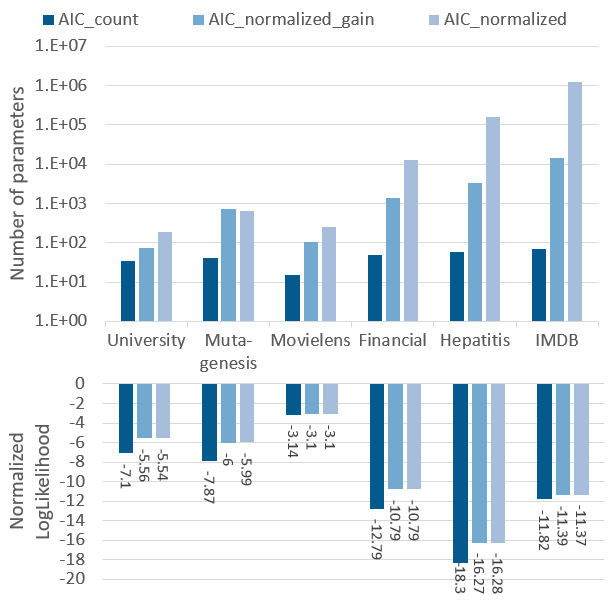
\includegraphics[width=0.5\textwidth] 
	{aicPlot.png}
	\centering
	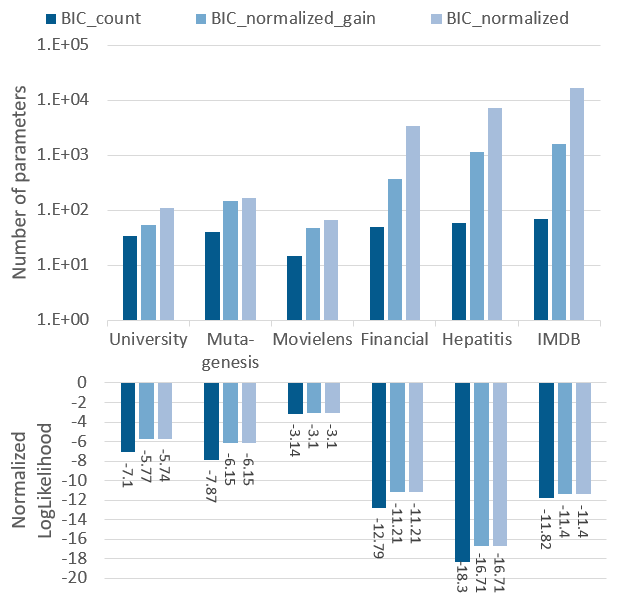
\includegraphics[width=0.5\textwidth] 
	{bicPlot.png}
	\caption{KLD with database distribution and Number of Parameters for different relational score upgrade methods. The number of parameters is shown on log-scale. Top: $\aic$ upgrades. Bottom: $\bic$ upgrades.
		\label{fig:scores}}
\end{figure}


\begin{figure}[thbp]
	\centering
	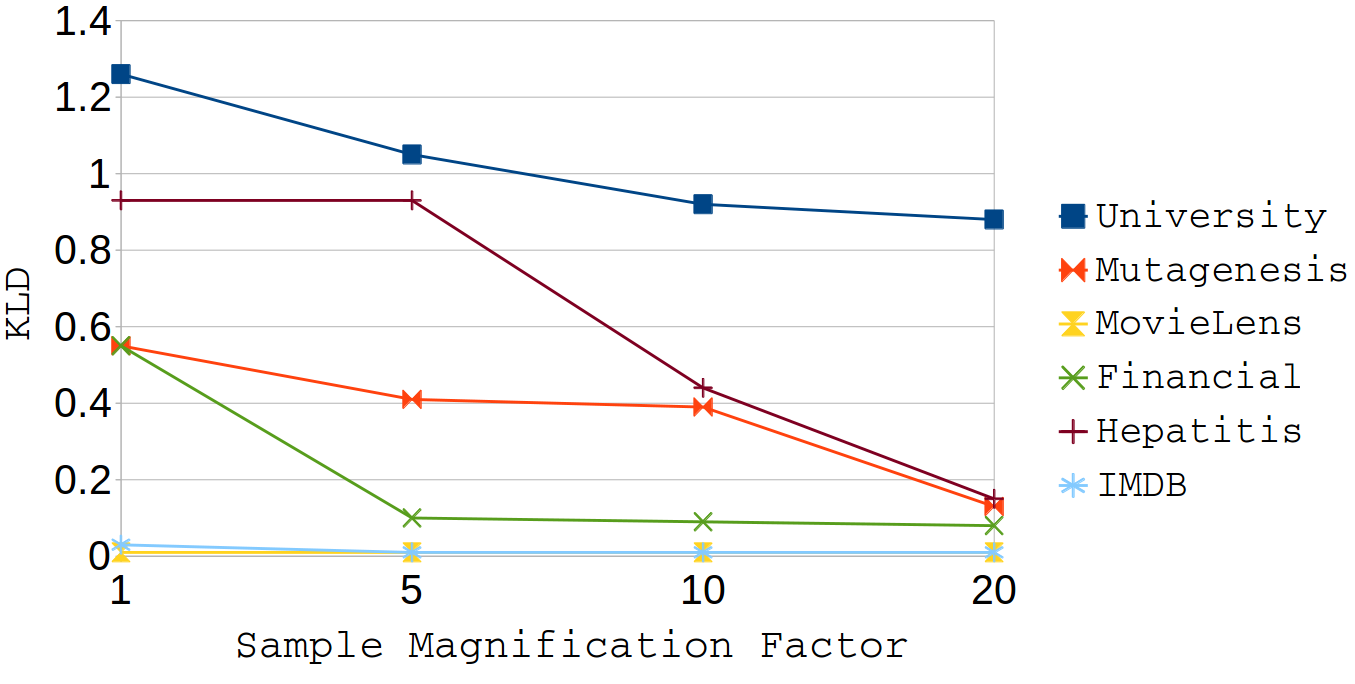
\includegraphics[width=0.5\textwidth] 
	{kld_count.png}
	\caption{KLD for the BIC count-count score \label{fig:kld_count}}
\end{figure}

\begin{figure}[thbp]
	\centering
	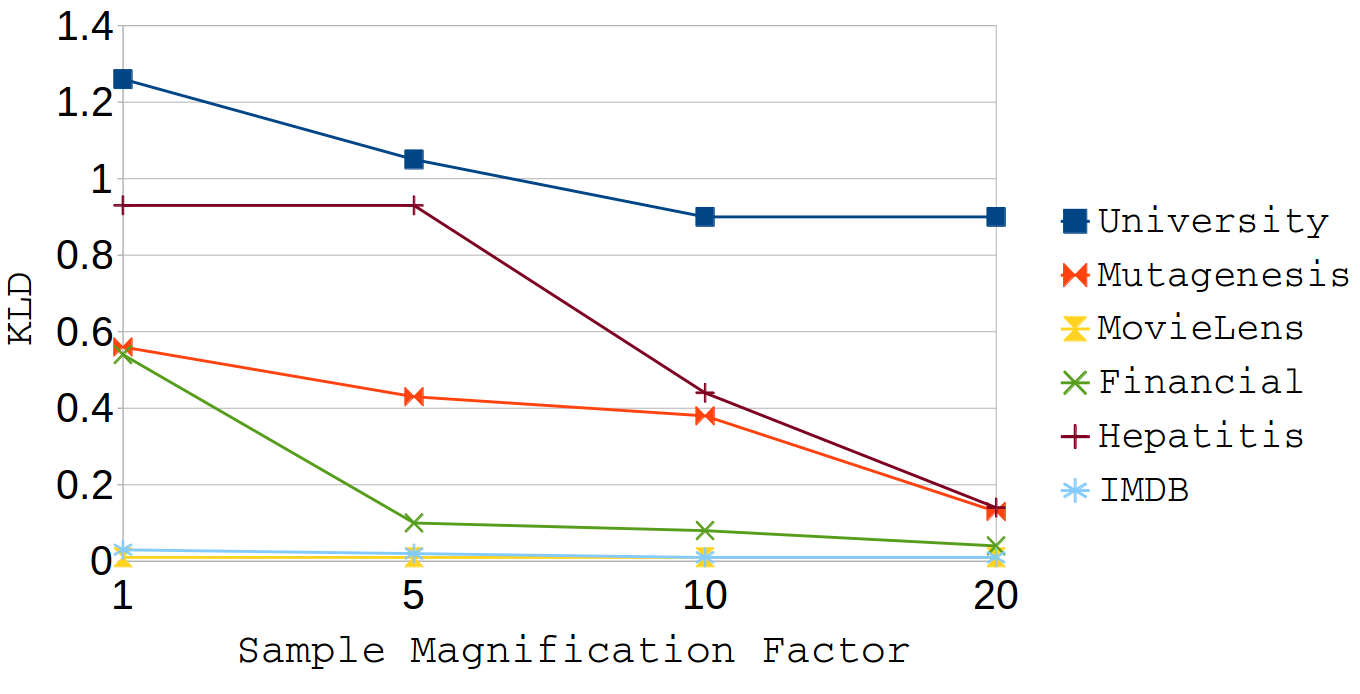
\includegraphics[width=0.5\textwidth] 
	{kld_ng.png}
	\caption{KLD for the BIC normalized gain \label{fig:kld_ng}}
\end{figure}

\subsubsection{Large Sample Size Comparison for the Count-Count and Normalized-Gain Methods} Recall that the count-count score uses the grounding count for the likelihood function and the number of parameters for the penalty term. The KLD of both upgrade methods is very close on all datasets. On MovieLens and Financial, the AIC count-count score uses more parameters than the normalized gain function, and on IMDb it uses fewer. On Hepatitis, the BIC count-count score uses significantly fewer parameters.

Figures~\ref{fig:kld_count} and~\ref{fig:kld_ng} consider the structures learned with increasing sample size. The figures are constructed as follows. We duplicate entities by a factor of $m = 1, 5, 10, 20.$ For example on IMDb, there would be 20 copies of BraveHeart with the same attributes and relationships. This can be viewed as a sampling-with-replacement variation of the design in \cite{Getoor2001,Schulte2014}, where the input database is also treated as representing a complete population. In terms of the model comparison scores, the local sample sizes are multiplied by a uniform {\em magnification factor}, which we denote as $\set{\samplesize} \times m$. 

As the magnification factor $m$ increases, the sample size tends towards infinity. 
The measurements reported therefore also illustrate the consistency analysis of Section~\ref{sec:theory}. To simplify the presentation, we focus on the BIC score. Unlike the AIC score~\cite[Sec.6.7]{Williams2001}, the BIC score is consistent for i.i.d. data~\cite{Chickering2002}. Therefore  Theorem~\ref{th:consistency} entails that it is also consistent for multi-relational data when upgraded with the normalized gain method. Figure~\ref{fig:kld_ng} shows the convergence to the database distribution (KLD = 0) on our benchmark databases for the normalized-gain BIC upgrade. The University dataset requires a higher magnification factor for convergence as the original dataset is much smaller than the others. The count-count score converges to the database distribution at a similar rate (Figure~\ref{fig:kld_count}). The exception is the Financial database where the count-count score stops improving at KLD = 0.08, compared to KLD = 0.04 for the normalized gain with sample magnification 20. While the KLD values are similar for the two upgrade methods (except for Financial), there are differences in the structures learned that we discuss next.




\paragraph{Edges Selected by the Normalized Gain Method but not by the Count-Count scores} 

Figure~\ref{fig:add-edges} fully confirms Hypothesis~\ref{hyp:noadd}: {\em the count-count BIC score selects no edges that add population variables.}  Together, Figures~\ref{fig:add-edges} and~\ref{fig:scores} confirm Hypothesis~\ref{hyp:contained}: whenever the normalized gain BIC upgrade find no such edges, it discovers the same structure as the count-count BIC upgrade (databases University and Mutagenesis). The fact that the count-count BIC score does not select dependencies represented by edges that add population variables, even with increasing sample size illustrates its nonconsistency.\footnote{\textbf{Sajjad}: add BIC expanding edges for count-count and normalized-normalized. Do this at magnification = 1. Normalized-gain should have goldilocks property.}



\begin{figure}[htbp]
	\centering
	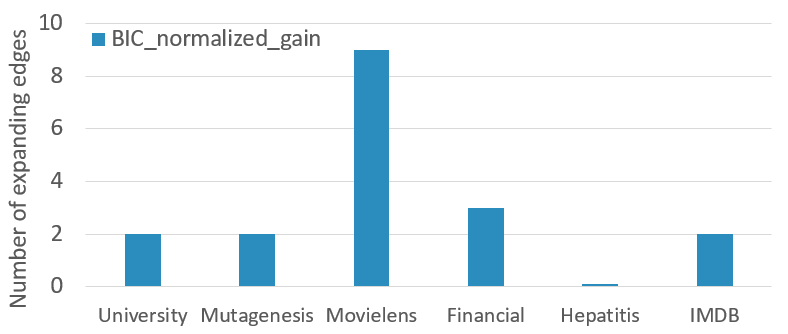
\includegraphics[width=0.5\textwidth] 
	{noEE.png}
	\caption{The number of edges that add population variables, for the normalized gain upgrade method. This number is 0 for the count-count method on every dataset. (Sample sizes magnified by a factor of 20).
		\label{fig:add-edges}}
\end{figure}


To understand the additional edges selected by the normalized gain BIC further, we assessed them in the light of domain knowledge. Figure~\ref{fig:example-edges} shows some of the plausible edges discovered by the Normalized BIC gain score with a magnification of 20. University: The grade of a student in a random course predicts her intelligence. MovieLens: The rating that a user assigns to a random movie predicts his or her gender and age. IMDb: If an actor appears in a movie whose language is English, she is more likely to be rated as high quality. UW: The years of a person in the program are predicted by whether his advisor has a position.
\begin{figure*}
	\centering
	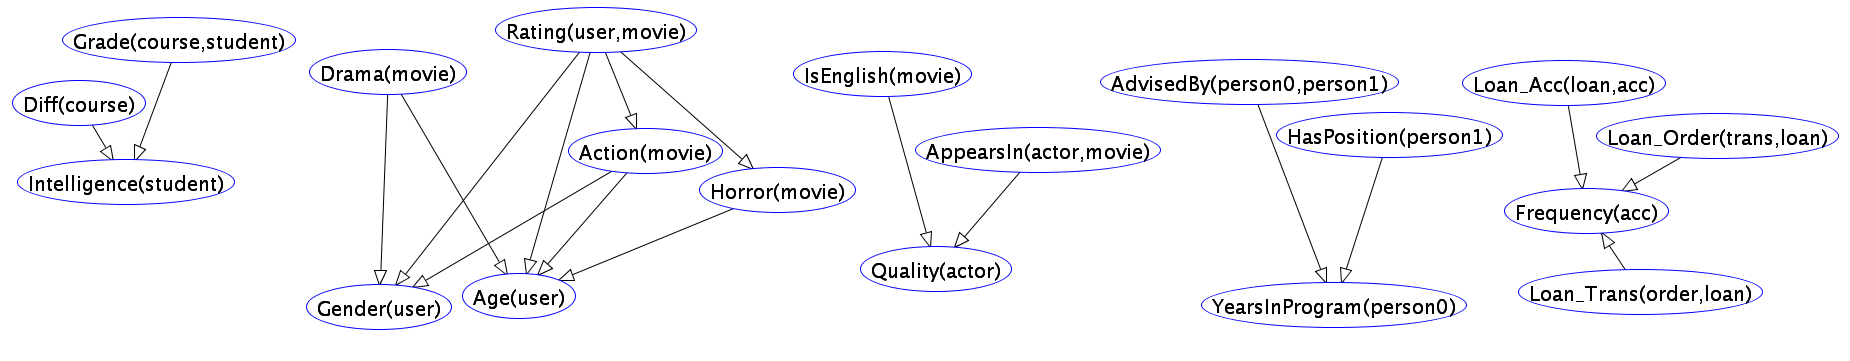
\includegraphics[width=1\textwidth] 
	{expandingEdges.png}
	\caption{Examples of edges selected by the normalized gain function that introduce additional population variables. Left to right: University, MovieLens, IMDb, Mutagenesis, Financial.  \label{fig:example-edges}}
\end{figure*}
Financial: The frequency of transactions for an account is predicted by facts about loans associated with the account. Based on domain understanding, it is plausible that these dependencies reflect genuine associations in the domain. However, the count-count method is incapable of finding them. 

\paragraph{Why Do Few Edges Add Population Variables?}

Figure~\ref{fig:add-edges} shows that the normalized gain function selects few edges that add population variables even in the sample size limit. The reason for this is that our datasets contain many unary attributes and relatively few binary functors that represent relationships. {\em If two unary attributes contain different population variables, they are marginally independent.} For example, the nodes $\it{gender}(\it{Actor})$ and $\it{genre}(\it{Movie})$ are marginally independent because the attributes of a randomly selected actor are independent of those of a randomly selected movie. The nodes may be conditionally dependent given that the actor appeared in the movie, that is, given $\it{AppearsIn}(\it{Actor},\it{Movie}) = \true$. However, a BN score tends to penalize edges that connect marginally independent nodes. Instead, it favors a v-structure $$\it{gender}(\it{Actor}) \rightarrow \it{AppearsIn}(\it{Actor},\it{Movie}) \leftarrow \it{genre}(\it{Movie})$$ for representing this (in)dependence pattern. No edge in this v-structure adds population variables. This observation shows another reason why adding population variables is helpful: once such an edge $\node_{+} \rightarrow \node$ is added, unary attributes can become conditionally dependent given $\node_{+}$. For example, once $\it{Rating(User,Movie)}$ is added as a parent of $\it{gender(User)}$, the relevance of $\it{Drama(Movie)}$ is assessed conditional on the fact that the user has rated the movie.


%
%Figure~\ref{fig:add-edges} also confirms Hypothesis~\ref{hyp:contained-most}: relatively few edges add population variables. From Figure~\ref{fig:scores}, the impact of these edges appears to be mixed. On MovieLens, they improve the log-likelihood score, whereas on IMDb and Hepatitis, the log-likelihood score is worse. Given that log-likelihood scores are close in all cases, and that the LAJ algorithm is a heuristic that may not return a global optimum, these findings are not conclusive against either upgrade method.




\paragraph{Conclusions} The experimental results support the normalized gain as the best upgrade method. The normalized-normalized and normalized-count upgrade methods are clearly inadequate. The count-count method is incapable of selecting edges that add population variables. We provided qualitative evidence that such edges can be informative. While the quantitative statistical evidence for their importance is mixed on our datasets, such a strong a priori bias against certain types of edges is clearly undesirable. In addition, the normalized gain is the only upgrade method in our set that has the important properties of balance and (relative) consistency. 


\section{Related Work} \label{sec:related}


We review related work on model selection for i.i.d. and for relational data.\footnote{\textbf{Oliver}: add tree diagram.}

\subsection{BN Model Selection for i.i.d. data}

Model selection criteria are a major topic in statistics \cite{Williams2001}. Model selection criteria for BN learning are a classic topic in machine learning; for review see~%\cite{Heckerman1998,bouckaert95:_bayes} . 
\cite{bouckaert95:_bayes}.
Our work extends the theoretical analysis of BN learning to multi-relational data. 


\subsection{BN Model Selection for Multi-Relational data} 
%For i.i.d. data, there is a unique likelihood function that measures the fit of a BN structure for a data set. 
For relational data, a likelihood function requires aggregating model probabilities for multiple instances of the template BN~\cite{Kimmig2014}. A number of different aggregation mechanisms have been proposed, resulting in different BN likelihood functions. 

\subsubsection{Likelihood based on Random Instantiations}
%The most recent proposal is the {\em random selection pseudo log-likelihood}
%~\cite{Schulte2011}. 
%Consider a randomly selected grounding of {\em all} population variables in a BN. Given a database, a single grounding determines a unique set of values for all nodes, and hence a unique log-likelihood via Equation~\eqref{eq:bn}. 
The {\em random selection log-likelihood score} is defined as the expected log-likelihood from a random grounding~\cite{Schulte2011}.
The random selection log-likelihood can be seen as an application of Halpern's well-known random selection semantics for first-order probabilistic logic~\cite{Halpern90}. 
The frequency log-likelihood of Table~\ref{table:ll} is a closed form for the random selection log-likelihood \cite[Prop.4.1]{Schulte2012}. For model selection, \cite{Schulte2012} suggests using what we call the normalized-count score, but does not investigate model selection scores in detail.

\subsubsection{Likelihood based on Complete Instantiations} This type of likelihood is based on  unrolling or grounding the BN~\cite{Heckerman+al:SRL07,Neville2007,Poole2003}. An inference graph contains all possible instances of edges in the first-order template, obtained by replacing population variables with constants. The inference model defines a conditional probability $P(\node_{ij}|\Pa{ij}{\graph})$, where $\node_{ij}$ denotes the $j$-th grounding of node $i$ in the template BN. This conditional probability aggregates the information from the multiple parent instances of the ground node $\node_{ij}$. Assuming that the ground inference graph is acyclic, a log-likelihood function can be defined by the usual BN formula 

\begin{equation}
\Score{\loglikelihood}{\graph}{\dstructure} \equiv \sum_{i} \sum_{j}^{\groundnode{i}}\ln P(\node_{ij}|\Pa{ij}{\graph}).
\end{equation}
 
There are two main approaches for defining the conditional probability model $P(\node_{ij}|\Pa{ij}{\graph})$, depending on how multiple instances of the same parent configuration are included~\cite{Natarajan2008}: Using (1) aggregate functions~\cite{Getoor2007c} and (2) combining rules~\cite{Kersting2007}. Model selection scores have been defined for both aggregators \cite{Getoor2007c} and combining rules. To our knowledge, the consistency of these model selection scores has not been investigated. Another open problem  with the complete instantiation approach is that the ground inference graph may contain cycles even if the template BN structure does not~\cite{Lowd2007}. 

%Since this appears to be an open problem, we briefly comment on how our analysis may be extended to other Bayesian network model selection scores. Since the product likelihood aggregates/combines multiple parents {\em before} multiplication, the local sample size associated with FORV $\node_{i}$ is $\groundnode_{i}$. This is independent of the model structure, therefore balancing is not a problem. 

% 
%
%[they are balanced: local sample size is number of groundings] 

Previous application of the Learn-and-Join algorithm \cite{Schulte2012} used a BN learner for i.i.d. data as a subroutine for learning a first-order BN. Combined with a log-linear prediction model, the features in the learned BN provide accurate predictions for the values of ground terms. While this upgrades BN learning algorithms, it does not upgrade i.i.d. model comparison criteria. In this paper we combine the LAJ search strategy with upgraded i.i.d. model scores.

\subsection{Markov Logic Networks}
A Markov Logic Network (MLN)  can be viewed as a template model for an {\em  un}directed graph.
\subsubsection{Model Selection} 
%Model selection scores have been researched for Markov Logic Networks (MLNs).  
%A Markov Logic Network (MLN) is a set of formulas $\mln=\{(\formula_{1},\w_{1}),\ldots,(\formula_{\numformulas},\w_{\numformulas})\}$ where $\formula_{i}$ is a formula, and each $\w_{i}$ is a real number called the weight of $\formula_{i}$. The log-likelihood for an MLN is given by 
%
%\begin{equation}
%\Score{\loglikelihood}{\mln}{\dstructure} = \sum_{i} \Count{\formula_{i}}{\dstructure} \w_{i} - \ln Z_{\mln}
%\end{equation}
%
%where $\Count{\formula_{i}}{\dstructure}$ is the number of groundings of $\formula_{i}$ in the database $\dstructure$ and $Z_{\mln}$ is a normalization constant (partition function) that depends on the MLN $\mln$ but not on the data $\dstructure$. 
%First-order BNs can be translated into MLNs by the standard moralization method~\cite[12.5.3]{Domingos2007}: essentially, marry all co-parents and omit edge directions. The count log-likelihood (Table~\ref{table:ll}) is the MLN log-likelihood score of a moralized FOB without the data-independent normalization constant (partition function)~\cite{Schulte2011}. 
Because computing the normalization constant (partition function) for the log-linear MLN likelihood function  is generally intractable, Markov structure learning often optimizes the pseudo log-likelihood \cite{Lowd2007,Kok2005a}. This is the sum of the log-conditional probabilities of each ground node value, given the values of all other ground nodes. 
%
%This conditional probability is proportional to the product of the clique potentials containing the target node. 
Similar to our normalized log-likelihood scores, the weighted pseudo log-likelihood (WPLL) normalizes the pseudo log-likelihood counts of different target nodes $\node_{ij}$ by the total number  $\groundnode{i}$ of the groundings of template node $\node_{i}$.
% to balance the contributions of nodes with different number of groundings. 
Each weight is penalized with a Gaussian shrinkage prior. The closest counterpart in our experiments is the normalized-count $\aic$ score of Table~\ref{table:comparison-scores}. The WPLL+penalty score is not consistent for the same reason as the normalized-count $\aic$ score. 
%Our theoretical analysis suggests that dividing the parameter penalty term by $\groundnode{i}$ as well would lead to a consistent score, and also improve predictive accuracy on test sets. 
%Given the close correspondence between log-linear scores for first-order Bayesian networks and MLNs, a promising avenue for future research is adapting the  approach in this paper for MLNs.

\subsubsection{Parameter Estimation} Xiang and Neville \cite{Xiang2011} provide a sophisticated asymptotic analysis of parameter learning for MLNs, given locality assumptions about the correlations between ground nodes. Our paper shares their framework of learning from one network. Similar to our paper, they consider a normalized log-likelihood score. Their main theorem shows that maximizing either the normalized log-likelihood or the pseudo log-likelihood leads to consistent parameter estimates. Different from our paper, they do not consider the consistency of MLN model selection.
%However, maximizing the log-likelihood is asymptotically more efficient (lower variance of estimates). Given the close correspondence between our likelihood functions of Table~\ref{table:ll} and the MLN log-likeihood, this suggests that these likelihood functions will lead to better parameter estimates than pseudo log-likelihood estimates. Extending the analysis of  \cite{Xiang2011} to model selection is a promising avenue for future research. 



\subsection{Other Models} 
The Inductive Logic Programming FOIL system \cite{foil} defined the information gain that results from adding a new condition (literal) to a first-order rule. The first-order information gain is similar to our approach in that 1) it defines a gain function rather than a score, and 2) the key issue concerns adding population variables. It is different in that 1) it is applied with discriminative models (classification), rather than generative models, and 2) different rule groundings are combined using existential quantification rather than a log-linear model.

A popular approach to modelling relational data is to learn latent factors such that links are independent of each other given the latent factors. 
%
%For example, a block model clusters entities such that the existence of a link between two entities depends on the cluster memberships of each. 
Sakai and Yamanishi 
\cite{Sakai2013} provide an asymptotic analysis of relational clustering when the number of clusters is selected to optimize normalized minimum description length. In this paper we did not consider latent factor learning, so our consistency result is not derived from conditional independence assumptions.


%\subsection{FOIL Gain}
%
%Similar in that it's a gain function, and focuses on expanding edges. Different in that it's for classification and uses existential quantification instead of a log-linear model.



\section{Conclusion and Future Work} We described a novel method for upgrading an i.i.d. Bayesian network score for multi-relational data. The normalized gain function measures the difference in data fit between two structures. Normalized gain functions preserve two key properties of i.i.d. BN scores: consistency and balance, meaning that the model's data likelihood  and the model's complexity are measured on the same scale. A surprising negative result is that these properties cannot be achieved with log-linear likelihood scores that are a function of a single model only. Empirical results demonstrate a special strength of the normalized gain upgrade method:  finding arcs whose source node contains population variables that are not included in the child node (e.g. $\it{Rating(User,Movie)} \rightarrow \it{age(User)}$). 

A promising avenue for future work is to extend our approach to other statistical-relational models that use complete instantiation likelihoods (see Section~\ref{sec:related}). It should be possible to develop a gain function for the log-linear likelihood of Markov Logic Networks. As for other Bayesian network relational models, Kersting and deRaedt suggest translating aggregation-based likelihoods into (the equivalent of) a FOB by adding complex aggregate terms as nodes~\cite{Kersting2007}. 
Recent results on representing combining rules in a logistic regression model suggest that similar complex terms can be defined  for combining rules~\cite{Buchman2015}. 
%Since our theoretical analysis makes no assumptions about the internal structure of the first-order random variables, it would also apply to Bayesian networks that include complex terms for representing aggregation or combining rules. 
Adding nodes that represent complex terms is a promising approach to unifying our framework with aggregate functions/combining rules. This has the potential to address both the question of consistency and the issue of cyclicity. 
%Another important way to expand the space of relational patterns beyond what we examined in this paper is to consider first-order terms that contain constants. 

Generalizing i.i.d. model selection scores designed for i.i.d. data is an important yet complex topic for relational learning. The normalized gain is a novel upgrade method that preserves important theoretical properties of i.i.d. model selection scores, and shows good empirical performance. 




%\section{References}\


\bibliographystyle{plain}
\bibliography{master}

\end{document}

$
\aiclocal{\graph}{i}{\dstructure} \equiv \dlogcount{\graph}{i}{\dstructure} - \numpars{\graph}{i}
$	&
$\aicimprove{\graph}{\graph'}{i}{\dstructure} \equiv \frac{\dlogcount{\graph'}{i}{\dstructure}}{\Fcount{\graph'}{i}{\dstructure}} - 
\frac{\frac{\Fcount{\graph'}{i}{\dstructure}}{\Fcount{\graph}{i}{\dstructure}}\dlogcount{\graph}{i}{\dstructure}}{\Fcount{\graph'}{i}{\dstructure}} + \frac{\numpars{\graph'}{i} - \numpars{\graph}{i}}{\Fcount{\graph'}{i}{\dstructure}}$

\begin{equation*}
\dlogcount{\graph}{i}{\dstructure} \equiv \sum_{j} \sum_{k} \ln \left( \frac
{\Fcount{\graph}{ijk}{\dstructure}}
{\Fcount{\graph}{ij}{\dstructure}}\right) \cdot \Fcount{\graph}{ijk}{\dstructure}
\end{equation*}

\begin{equation*}
\aiclocal{\graph}{i}{\dstructure} \equiv \dlogcount{\graph}{i}{\dstructure} - \numpars{\graph}{i}
\end{equation*}

\begin{equation*}
\logimprove{\graph}{\graph'}{i}{\dstructure} \equiv \frac
{\Fcount{\graph'}{i}{\dstructure}}
{\Fcount{\graph}{i}{\dstructure}}
\dlogcount{\graph}{i}{\dstructure} - \dlogcount{\graph'}{i}{\dstructure}
\end{equation*}

\begin{equation*}
\aicimprove{\graph}{\graph'}{i}{\dstructure} \equiv \logimprove{\graph}{\graph'}{i}{\dstructure} - \numpars{\graph}{i} + \numpars{\graph'}{i}
\end{equation*}

\begin{equation*}
\biclocal{\graph}{i}{\dstructure} \equiv \dlogcount{\graph}{i}{\dstructure} - log(\numpars{\graph}{i})
\end{equation*}


\begin{equation*}
\bicimprove{\graph}{\graph'}{i}{\dstructure} \equiv \logimprove{\graph}{\graph'}{i}{\dstructure} - log(\numpars{\graph}{i}) + log(\numpars{\graph'}{i})
\end{equation*}
